\chapter{Detailed design}

In this chapter, every single code object is described in terms of public
interface and functionality. Because of the fairly dynamic character of this
project -- new ideas come and go -- this chapter will not be finished until the
end of the project and will probably change regularly.

\section{Files and directories}

All source code will be in the directory \texttt{src/}. All classes are in the
package \texttt{amber} or in a subpackage thereof. The Psyclone specification
file \texttt{psySpec.xml} is found in \texttt{data/}. External libraries that
are redistributed with \Amber\ are in \texttt{lib/}. The source of this
document, the traineeship report and the website are located in
\texttt{documentation/}.

The application is written using
Eclipse\footnote{\url{http://www.eclipse.org/}} and can be built using Apache
Ant\footnote{\url{http://ant.apache.org/}}. It requires Java SDK version 1.5 or
greater.

To open the project in Eclipse, the following user libraries need to be
defined: ``Informa RSS Library'' and ``Jakarta Commons CLI''. These are the
only two depending libraries which aren't redistributed with \Amber\, the first
is a redistribution of a collection of libaries already to be found at
\url{http://informa.sourceforge.net/}, while the other is readily available at
\url{http://jakarta.apache.org/commons/cli/}.

\section{Classes}

Since the project is written in Java, the code objects are classes. This
section deals mainly with the relation between the class hierarchies and their
function.

\subsection{Module class hierarchy}

The Module family is the collection of classes which can perform a production
task within the \Amber\ system. They are the most important family of objects.
The first distinction is the general functionality: crawling, analysing and
visualising.

Secondly, as there can be more than one means to do one of the three main
tasks, a class can extend one of these main modules. Thus we get the UML
inheritance model as displayed in Figure~\ref{fig:class-diagram-module}.

\begin{figure}[htp]
  \centering
  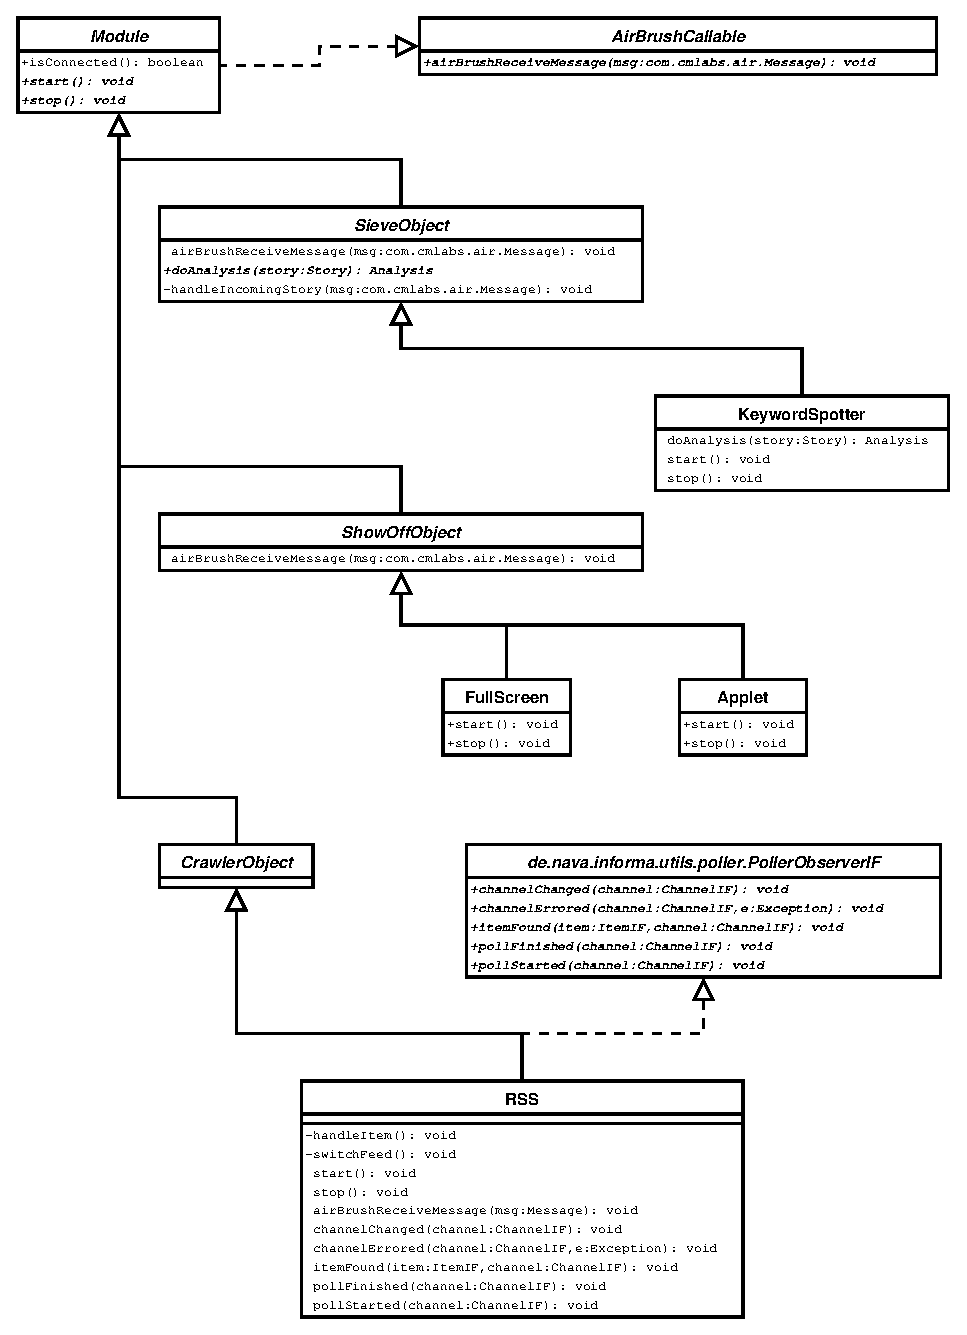
\includegraphics{design/image/class-diagram-module}
  \caption{
    \label{fig:class-diagram-module}
    The inheritance model of the Module class}
\end{figure}

\subsection{AmberMessage class hierarchy}

AmberMessage objects are the holders of information sent and received via
Psyclone. They provide means of (de)serializing data to and from Psyclone and
in this way are a abstraction of the raw messages to the level of Java.

There are two subclasses of AmberMessage, Story and Analysis, which are to be
used for posting on the WB.Stories and WB.Analyses whiteboards respectively.

A Module can introduce extra subclasses if it needs so for sending and
receiving configuration data over Psyclone.

The UML inheritance model is shown in
Figure~\ref{fig:class-diagram-ambermessage}.

\begin{figure}[htp]
  \centering
  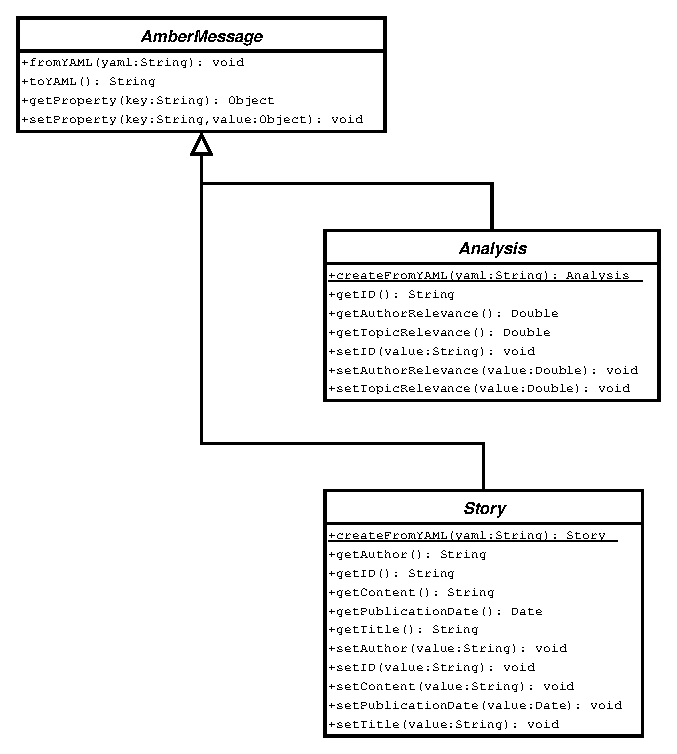
\includegraphics{design/image/class-diagram-ambermessage}
  \caption{
    \label{fig:class-diagram-ambermessage}
    The inheritance model of the AmberMessage class}
\end{figure}

\subsection{Other classes}

There are classes which directly descend from the Java Object class and are as
such outside the \Amber\ hierarchy. They are displayed in
Figure~\ref{fig:class-diagram}.

The first is the Particle class, it represents a particle in the visualisation
module. It is initialized to be ``on the surface of the earth'', then launch
parameters are set according to the result of the first analysis which came in
and it is launched. It will calculate its new position when the visualiser
requests so.

Another class is the AirBrush class, which eases communication with the Java
OpenAIR library.

The Launcher is a class which provides an interface to the command line and is
responsible for starting and stopping the program. It has a command line
argument parser which makes unwanted hard coding of parameters largely
unneccesary.

Lastly, there is the EarthView class which is a Swing component to be placed in
a window, which will draw Particles as they orbit around the earth.

\begin{figure}[htp]
  \centering
  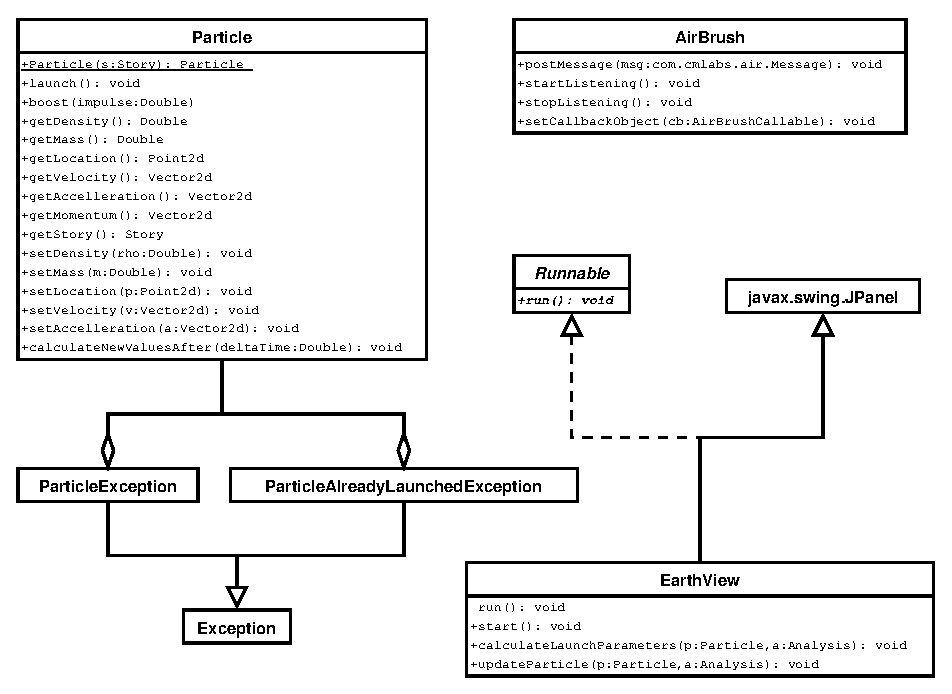
\includegraphics{design/image/class-diagram}
  \caption{
    \label{fig:class-diagram}
    The inheritance model of the remaining classes}
\end{figure}

\section{Detailed class descriptions}

The next sections describe all classes in more detail, based on their location
in the code base. The descriptions were automatically extracted from the
sources via Javadoc and the \TeX{}Doclet.

      \vspace{1mm}%
\subsection{Package amber}{
\label{amber}\hbox to \hsize{\it Package Contents\hfil Page}
\vskip .13in
\hbox{\bf Classes}
\entityintro{Crawler}{amber.Crawler}{Gathers information, be it from the internet or from another information system.}
\entityintro{ShowOff}{amber.ShowOff}{Displays the information available in the whiteboards.}
\entityintro{Sieve}{amber.Sieve}{Provides a means of adding meaning to a story.}
\vskip .1in
\vskip .1in
\subsubsection{\label{amber.Crawler}\index{Crawler}Class Crawler}{
\vskip .1in 
Gathers information, be it from the internet or from another information system. They post Story messages to a Psyclone whiteboard.\vskip .1in 
\subsubsection{Declaration}{
\small public abstract class Crawler
\\ {\bf extends} amber.common.Module
\refdefined{amber.common.Module}}
\subsubsection{All known subclasses}{RSS\small{\refdefined{amber.crawler.RSS}}}
\subsubsection{Constructors}{
\vskip -2em
\begin{itemize}
 \item{ 
\index{Crawler(String, String, Integer)}
{\bf Crawler}\\
{\tt public\ {\bf Crawler}( {\tt java.lang.String} {\bf moduleName},
{\tt java.lang.String} {\bf hostname},
{\tt java.lang.Integer} {\bf port} )
\label{amber.Crawler(java.lang.String, java.lang.String, java.lang.Integer)}}%end signature
\begin{itemize}
\item{
{\bf Parameters}
  \begin{itemize}
   \item{
{\tt moduleName} -- the name of the module to start}
   \item{
{\tt hostname} -- hostname of the psyclone server}
   \item{
{\tt port} -- port of the psyclone server}
  \end{itemize}
}%end item
\end{itemize}
}%end item
\end{itemize}
}
}
\subsubsection{\label{amber.ShowOff}\index{ShowOff}Class ShowOff}{
\vskip .1in 
Displays the information available in the whiteboards. They combine Story messages with Analysis messages. It is dependent on the type of visualization one wants to accomplish what will be displayed and in what manner.\vskip .1in 
\subsubsection{Declaration}{
\small public abstract class ShowOff
\\ {\bf extends} amber.common.Module
\refdefined{amber.common.Module}}
\subsubsection{All known subclasses}{EarthViewWrapper\small{\refdefined{amber.showoff.EarthViewWrapper}}, FullScreen\small{\refdefined{amber.showoff.FullScreen}}}
\subsubsection{Fields}{
\begin{itemize}
\item{
\index{storyQueue}
\label{amber.ShowOff.storyQueue}protected showoff.ObservableList {\bf storyQueue}\begin{itemize}
\item{\vskip -.9ex 
In this list incoming stories are stored before they are handled.}
\end{itemize}
}
\item{
\index{analysisQueue}
\label{amber.ShowOff.analysisQueue}protected showoff.ObservableList {\bf analysisQueue}\begin{itemize}
\item{\vskip -.9ex 
In this list incoming analyses are stored before they are handled.}
\end{itemize}
}
\item{
\index{STORY\_LIFETIME}
\label{amber.ShowOff.STORY_LIFETIME}private int {\bf STORY\_LIFETIME}}
\end{itemize}
}
\subsubsection{Constructors}{
\vskip -2em
\begin{itemize}
 \item{ 
\index{ShowOff(String, String, Integer)}
{\bf ShowOff}\\
{\tt public\ {\bf ShowOff}( {\tt java.lang.String} {\bf moduleName},
{\tt java.lang.String} {\bf hostname},
{\tt java.lang.Integer} {\bf port} )
\label{amber.ShowOff(java.lang.String, java.lang.String, java.lang.Integer)}}%end signature
\begin{itemize}
\item{
{\bf Parameters}
  \begin{itemize}
   \item{
{\tt moduleName} -- the name of the module to start}
   \item{
{\tt hostname} -- hostname of the psyclone server}
   \item{
{\tt port} -- port of the psyclone server}
  \end{itemize}
}%end item
\end{itemize}
}%end item
\end{itemize}
}
\subsubsection{Methods}{
\vskip -2em
\begin{itemize}
 \item{ 
\index{airBrushReceiveMessage(Message)}
{\bf airBrushReceiveMessage}\\
{\tt  boolean\ {\bf airBrushReceiveMessage}( {\tt com.cmlabs.air.Message} {\bf msg} )
\label{amber.ShowOff.airBrushReceiveMessage(com.cmlabs.air.Message)}}%end signature
\begin{itemize}
\item{
{\bf Description copied from common.AirBrushCallable{\small \refdefined{amber.common.AirBrushCallable}} }

Message reception handler. It is called on the object implementing this interface which was set in AirBrush.
}
\item{
{\bf Parameters}
  \begin{itemize}
   \item{
{\tt msg} -- }
  \end{itemize}
}%end item
\item{{\bf Returns} -- 
true if the message was handled, false if it wasn't 
}%end item
\item{{\bf See also}
  \begin{itemize}
\item{ {\tt common.AirBrush.setCallbackObject(AirBrushCallable)} {\small 
\refdefined{amber.common.AirBrush.setCallbackObject(amber.common.AirBrushCallable)}}%end
}
  \end{itemize}
}%end item
\end{itemize}
}%end item
 \item{ 
\index{start()}
{\bf start}\\
{\tt public void\ {\bf start}(  )
\label{amber.ShowOff.start()}}%end signature
\begin{itemize}
\item{
{\bf Description copied from common.Module{\small \refdefined{amber.common.Module}} }

Start normal operation after initialization and configuration
}
\end{itemize}
}%end item
\end{itemize}
}
}
\subsubsection{\label{amber.Sieve}\index{Sieve}Class Sieve}{
\vskip .1in 
Provides a means of adding meaning to a story. When a Story message comes in, the Sieve module will generate an Analysis based on it.\vskip .1in 
\subsubsection{Declaration}{
\small public abstract class Sieve
\\ {\bf extends} amber.common.Module
\refdefined{amber.common.Module}}
\subsubsection{All known subclasses}{KeywordSpotter\small{\refdefined{amber.sieve.KeywordSpotter}}}
\subsubsection{Fields}{
\begin{itemize}
\item{
\index{topicString}
\label{amber.Sieve.topicString}protected java.lang.String {\bf topicString}\begin{itemize}
\item{\vskip -.9ex 
topic this Sieve creates Analyses for}
\end{itemize}
}
\item{
\index{messageTypeSuffix}
\label{amber.Sieve.messageTypeSuffix}private final java.lang.String {\bf messageTypeSuffix}\begin{itemize}
\item{\vskip -.9ex 
the suffix of messages to be sent to the whiteboard}
\end{itemize}
}
\end{itemize}
}
\subsubsection{Constructors}{
\vskip -2em
\begin{itemize}
 \item{ 
\index{Sieve(String, String, Integer)}
{\bf Sieve}\\
{\tt public\ {\bf Sieve}( {\tt java.lang.String} {\bf name},
{\tt java.lang.String} {\bf hostname},
{\tt java.lang.Integer} {\bf port} )
\label{amber.Sieve(java.lang.String, java.lang.String, java.lang.Integer)}}%end signature
\begin{itemize}
\item{
{\bf Parameters}
  \begin{itemize}
   \item{
{\tt name} -- the name of the module to start}
   \item{
{\tt hostname} -- hostname of the psyclone server}
   \item{
{\tt port} -- port of the psyclone server}
  \end{itemize}
}%end item
\end{itemize}
}%end item
\end{itemize}
}
\subsubsection{Methods}{
\vskip -2em
\begin{itemize}
 \item{ 
\index{airBrushReceiveMessage(Message)}
{\bf airBrushReceiveMessage}\\
{\tt  boolean\ {\bf airBrushReceiveMessage}( {\tt com.cmlabs.air.Message} {\bf msg} )
\label{amber.Sieve.airBrushReceiveMessage(com.cmlabs.air.Message)}}%end signature
\begin{itemize}
\item{
{\bf Description copied from common.AirBrushCallable{\small \refdefined{amber.common.AirBrushCallable}} }

Message reception handler. It is called on the object implementing this interface which was set in AirBrush.
}
\item{
{\bf Parameters}
  \begin{itemize}
   \item{
{\tt msg} -- }
  \end{itemize}
}%end item
\item{{\bf Returns} -- 
true if the message was handled, false if it wasn't 
}%end item
\item{{\bf See also}
  \begin{itemize}
\item{ {\tt common.AirBrush.setCallbackObject(AirBrushCallable)} {\small 
\refdefined{amber.common.AirBrush.setCallbackObject(amber.common.AirBrushCallable)}}%end
}
  \end{itemize}
}%end item
\end{itemize}
}%end item
 \item{ 
\index{doAnalysis(Story)}
{\bf doAnalysis}\\
{\tt protected abstract common.Analysis\ {\bf doAnalysis}( {\tt common.Story} {\bf story} )
\label{amber.Sieve.doAnalysis(amber.common.Story)}}%end signature
\begin{itemize}
\item{
{\bf Parameters}
  \begin{itemize}
   \item{
{\tt story} -- the story to be analysed}
  \end{itemize}
}%end item
\item{{\bf Returns} -- 
a newly created Analysis object which contains information about the story 
}%end item
\end{itemize}
}%end item
 \item{ 
\index{handleIncomingStory(Message)}
{\bf handleIncomingStory}\\
{\tt protected void\ {\bf handleIncomingStory}( {\tt com.cmlabs.air.Message} {\bf msg} )
\label{amber.Sieve.handleIncomingStory(com.cmlabs.air.Message)}}%end signature
\begin{itemize}
\item{
{\bf Description}

an incoming message gets analysed, if it is deemed relevant the analysis immediately sent on
}
\item{
{\bf Parameters}
  \begin{itemize}
   \item{
{\tt msg} -- }
  \end{itemize}
}%end item
\end{itemize}
}%end item
\end{itemize}
}
}
}
\subsection{Package amber.common}{
\label{amber.common}\hbox to \hsize{\it Package Contents\hfil Page}
\vskip .13in
\hbox{\bf Interfaces}
\entityintro{AirBrushCallable}{amber.common.AirBrushCallable}{Specificies the callback functions for communication with AirBrush, the interface to JavaOpenAIR.}
\vskip .13in
\hbox{\bf Classes}
\entityintro{AirBrush}{amber.common.AirBrush}{A small layer between JavaOpenAIR and Amber.}
\entityintro{AmberMessage}{amber.common.AmberMessage}{Superclass of all messages that are serialized and sent to Psyclone.}
\entityintro{Analysis}{amber.common.Analysis}{Holds information about a single Story object.}
\entityintro{Launcher}{amber.common.Launcher}{To be called directly from the commandline and is in fact the preferred way to start any Amber module.}
\entityintro{Module}{amber.common.Module}{Parent class of all Amber modules.}
\entityintro{Polar2d}{amber.common.Polar2d}{Represents polar coordinates: Angle and distance from origin.}
\entityintro{Story}{amber.common.Story}{Holds all (meta-)information directly connected to a crawled story.}
\vskip .1in
\vskip .1in
\subsubsection{\label{amber.common.AirBrushCallable}\index{AirBrushCallable@{\it AirBrushCallable}}Interface AirBrushCallable}{
\vskip .1in 
Specificies the callback functions for communication with AirBrush, the interface to JavaOpenAIR.\vskip .1in 
\subsubsection{Declaration}{
\small public interface AirBrushCallable
}
\subsubsection{All known subinterfaces}{Sieve\small{\refdefined{amber.Sieve}}, ShowOff\small{\refdefined{amber.ShowOff}}, Crawler\small{\refdefined{amber.Crawler}}, Module\small{\refdefined{amber.common.Module}}, RSS\small{\refdefined{amber.crawler.RSS}}, EarthViewWrapper\small{\refdefined{amber.showoff.EarthViewWrapper}}, FullScreen\small{\refdefined{amber.showoff.FullScreen}}, KeywordSpotter\small{\refdefined{amber.sieve.KeywordSpotter}}}
\subsubsection{All classes known to implement interface}{Module\small{\refdefined{amber.common.Module}}}
\subsubsection{Methods}{
\vskip -2em
\begin{itemize}
 \item{ 
\index{airBrushReceiveMessage(Message)}
{\bf airBrushReceiveMessage}\\
{\tt  boolean\ {\bf airBrushReceiveMessage}( {\tt com.cmlabs.air.Message} {\bf msg} )
\label{amber.common.AirBrushCallable.airBrushReceiveMessage(com.cmlabs.air.Message)}}%end signature
\begin{itemize}
\item{
{\bf Description}

Message reception handler. It is called on the object implementing this interface which was set in AirBrush.
}
\item{
{\bf Parameters}
  \begin{itemize}
   \item{
{\tt msg} -- }
  \end{itemize}
}%end item
\item{{\bf Returns} -- 
true if the message was handled, false if it wasn't 
}%end item
\item{{\bf See also}
  \begin{itemize}
\item{ {\tt AirBrush.setCallbackObject(AirBrushCallable)} {\small 
\refdefined{amber.common.AirBrush.setCallbackObject(amber.common.AirBrushCallable)}}%end
}
  \end{itemize}
}%end item
\end{itemize}
}%end item
\end{itemize}
}
}
\subsubsection{\label{amber.common.AirBrush}\index{AirBrush}Class AirBrush}{
\vskip .1in 
A small layer between JavaOpenAIR and Amber. It holds state information about the connection with the Psyclone server and such.\vskip .1in 
\subsubsection{Declaration}{
\small public class AirBrush
\\ {\bf extends} java.lang.Object
\refdefined{java.lang.Object}\\ {\bf implements} 
java.lang.Runnable}
\subsubsection{Fields}{
\begin{itemize}
\item{
\index{plug}
\label{amber.common.AirBrush.plug}public final com.cmlabs.air.JavaAIRPlug {\bf plug}\begin{itemize}
\item{\vskip -.9ex 
the connection object}
\end{itemize}
}
\item{
\index{thread}
\label{amber.common.AirBrush.thread}private java.lang.Thread {\bf thread}\begin{itemize}
\item{\vskip -.9ex 
thread handling incoming messages}
\end{itemize}
}
\item{
\index{callback}
\label{amber.common.AirBrush.callback}private AirBrushCallable {\bf callback}\begin{itemize}
\item{\vskip -.9ex 
the callback object}
\end{itemize}
}
\item{
\index{moduleName}
\label{amber.common.AirBrush.moduleName}private java.lang.String {\bf moduleName}\begin{itemize}
\item{\vskip -.9ex 
the string containing the name of the running module}
\end{itemize}
}
\end{itemize}
}
\subsubsection{Constructors}{
\vskip -2em
\begin{itemize}
 \item{ 
\index{AirBrush(String, String, Integer)}
{\bf AirBrush}\\
{\tt public\ {\bf AirBrush}( {\tt java.lang.String} {\bf module},
{\tt java.lang.String} {\bf hostname},
{\tt java.lang.Integer} {\bf port} )
\label{amber.common.AirBrush(java.lang.String, java.lang.String, java.lang.Integer)}}%end signature
\begin{itemize}
\item{
{\bf Description}

Creates and initializes AirBrush and connects to the Psyclone server.
}
\item{
{\bf Parameters}
  \begin{itemize}
   \item{
{\tt module} -- the name of the module to connect}
   \item{
{\tt hostname} -- hostname of the Psyclone server}
   \item{
{\tt port} -- port number of the Psyclone server}
  \end{itemize}
}%end item
\end{itemize}
}%end item
\end{itemize}
}
\subsubsection{Methods}{
\vskip -2em
\begin{itemize}
 \item{ 
\index{getParameterDouble(String)}
{\bf getParameterDouble}\\
{\tt public java.lang.Double\ {\bf getParameterDouble}( {\tt java.lang.String} {\bf key} )
\label{amber.common.AirBrush.getParameterDouble(java.lang.String)}}%end signature
\begin{itemize}
\item{
{\bf Description}

Get the parameter with type Double
}
\item{
{\bf Parameters}
  \begin{itemize}
   \item{
{\tt key} -- }
  \end{itemize}
}%end item
\item{{\bf Returns} -- 
the parameter stored under key 
}%end item
\end{itemize}
}%end item
 \item{ 
\index{getParameterInteger(String)}
{\bf getParameterInteger}\\
{\tt public java.lang.Integer\ {\bf getParameterInteger}( {\tt java.lang.String} {\bf key} )
\label{amber.common.AirBrush.getParameterInteger(java.lang.String)}}%end signature
\begin{itemize}
\item{
{\bf Description}

Get the parameter with type Integer
}
\item{
{\bf Parameters}
  \begin{itemize}
   \item{
{\tt key} -- }
  \end{itemize}
}%end item
\item{{\bf Returns} -- 
the parameter stored under key 
}%end item
\end{itemize}
}%end item
 \item{ 
\index{getParameterString(String)}
{\bf getParameterString}\\
{\tt public java.lang.String\ {\bf getParameterString}( {\tt java.lang.String} {\bf key} )
\label{amber.common.AirBrush.getParameterString(java.lang.String)}}%end signature
\begin{itemize}
\item{
{\bf Description}

Get the parameter with type String
}
\item{
{\bf Parameters}
  \begin{itemize}
   \item{
{\tt key} -- }
  \end{itemize}
}%end item
\item{{\bf Returns} -- 
the parameter stored under key 
}%end item
\end{itemize}
}%end item
 \item{ 
\index{hasParameter(String)}
{\bf hasParameter}\\
{\tt public boolean\ {\bf hasParameter}( {\tt java.lang.String} {\bf key} )
\label{amber.common.AirBrush.hasParameter(java.lang.String)}}%end signature
\begin{itemize}
\item{
{\bf Parameters}
  \begin{itemize}
   \item{
{\tt key} -- }
  \end{itemize}
}%end item
\item{{\bf Returns} -- 
true when the parameter named key is present 
}%end item
\end{itemize}
}%end item
 \item{ 
\index{openWhiteboard(String)}
{\bf openWhiteboard}\\
{\tt public boolean\ {\bf openWhiteboard}( {\tt java.lang.String} {\bf wb} )
\label{amber.common.AirBrush.openWhiteboard(java.lang.String)}}%end signature
\begin{itemize}
\item{
{\bf Description}

Open connection a two-way connection with the whiteboard
}
\item{
{\bf Parameters}
  \begin{itemize}
   \item{
{\tt wb} -- name of the whiteboard to connect with}
  \end{itemize}
}%end item
\item{{\bf Returns} -- 
true if the whiteboard was succesfully opened 
}%end item
\end{itemize}
}%end item
 \item{ 
\index{postMessage(Message)}
{\bf postMessage}\\
{\tt public void\ {\bf postMessage}( {\tt com.cmlabs.air.Message} {\bf msg} )
\label{amber.common.AirBrush.postMessage(com.cmlabs.air.Message)}}%end signature
\begin{itemize}
\item{
{\bf Description}

Post a message to Psyclone
}
\item{
{\bf Parameters}
  \begin{itemize}
   \item{
{\tt msg} -- }
  \end{itemize}
}%end item
\end{itemize}
}%end item
 \item{ 
\index{run()}
{\bf run}\\
{\tt  void\ {\bf run}(  )
\label{amber.common.AirBrush.run()}}%end signature
}%end item
 \item{ 
\index{setCallbackObject(AirBrushCallable)}
{\bf setCallbackObject}\\
{\tt public void\ {\bf setCallbackObject}( {\tt AirBrushCallable} {\bf cb} )
\label{amber.common.AirBrush.setCallbackObject(amber.common.AirBrushCallable)}}%end signature
\begin{itemize}
\item{
{\bf Description}

Set the callback object for handling incoming messages
}
\item{
{\bf Parameters}
  \begin{itemize}
   \item{
{\tt cb} -- the callback object}
  \end{itemize}
}%end item
\item{{\bf See also}
  \begin{itemize}
\item{ {\tt AirBrushCallable} {\small 
\refdefined{amber.common.AirBrushCallable}}%end
}
  \end{itemize}
}%end item
\end{itemize}
}%end item
 \item{ 
\index{setParameter(String, Double)}
{\bf setParameter}\\
{\tt public void\ {\bf setParameter}( {\tt java.lang.String} {\bf key},
{\tt java.lang.Double} {\bf value} )
\label{amber.common.AirBrush.setParameter(java.lang.String, java.lang.Double)}}%end signature
\begin{itemize}
\item{
{\bf Description}

Set a parameter in Psyclone for the current module
}
\item{
{\bf Parameters}
  \begin{itemize}
   \item{
{\tt key} -- }
   \item{
{\tt value} -- }
  \end{itemize}
}%end item
\end{itemize}
}%end item
 \item{ 
\index{setParameter(String, Integer)}
{\bf setParameter}\\
{\tt public void\ {\bf setParameter}( {\tt java.lang.String} {\bf key},
{\tt java.lang.Integer} {\bf value} )
\label{amber.common.AirBrush.setParameter(java.lang.String, java.lang.Integer)}}%end signature
\begin{itemize}
\item{
{\bf Description}

Set a parameter in Psyclone for the current module
}
\item{
{\bf Parameters}
  \begin{itemize}
   \item{
{\tt key} -- }
   \item{
{\tt value} -- }
  \end{itemize}
}%end item
\end{itemize}
}%end item
 \item{ 
\index{setParameter(String, String)}
{\bf setParameter}\\
{\tt public void\ {\bf setParameter}( {\tt java.lang.String} {\bf key},
{\tt java.lang.String} {\bf value} )
\label{amber.common.AirBrush.setParameter(java.lang.String, java.lang.String)}}%end signature
\begin{itemize}
\item{
{\bf Description}

Set a parameter in Psyclone for the current module
}
\item{
{\bf Parameters}
  \begin{itemize}
   \item{
{\tt key} -- }
   \item{
{\tt value} -- }
  \end{itemize}
}%end item
\end{itemize}
}%end item
 \item{ 
\index{startListening()}
{\bf startListening}\\
{\tt public void\ {\bf startListening}(  )
\label{amber.common.AirBrush.startListening()}}%end signature
\begin{itemize}
\item{
{\bf Description}

Start listening for incoming messages
}
\end{itemize}
}%end item
 \item{ 
\index{stopListening()}
{\bf stopListening}\\
{\tt public void\ {\bf stopListening}(  )
\label{amber.common.AirBrush.stopListening()}}%end signature
\begin{itemize}
\item{
{\bf Description}

Stop listening and disconnect from Psyclone
}
\end{itemize}
}%end item
\end{itemize}
}
}
\subsubsection{\label{amber.common.AmberMessage}\index{AmberMessage}Class AmberMessage}{
\vskip .1in 
Superclass of all messages that are serialized and sent to Psyclone. Messages are serialized in YAML format.\vskip .1in 
\subsubsection{Declaration}{
\small public abstract class AmberMessage
\\ {\bf extends} java.lang.Object
\refdefined{java.lang.Object}}
\subsubsection{All known subclasses}{Story\small{\refdefined{amber.common.Story}}, Analysis\small{\refdefined{amber.common.Analysis}}, EarthViewStory\small{\refdefined{amber.showoff.EarthViewStory}}}
\subsubsection{Fields}{
\begin{itemize}
\item{
\index{storage}
\label{amber.common.AmberMessage.storage}private java.util.Hashtable {\bf storage}\begin{itemize}
\item{\vskip -.9ex 
storage of the properties}
\end{itemize}
}
\end{itemize}
}
\subsubsection{Constructors}{
\vskip -2em
\begin{itemize}
 \item{ 
\index{AmberMessage()}
{\bf AmberMessage}\\
{\tt public\ {\bf AmberMessage}(  )
\label{amber.common.AmberMessage()}}%end signature
}%end item
\end{itemize}
}
\subsubsection{Methods}{
\vskip -2em
\begin{itemize}
 \item{ 
\index{fromYAML(String)}
{\bf fromYAML}\\
{\tt public void\ {\bf fromYAML}( {\tt java.lang.String} {\bf in} )
\label{amber.common.AmberMessage.fromYAML(java.lang.String)}}%end signature
\begin{itemize}
\item{
{\bf Description}

Converts a String generated by toYAML() to the correct contents of the object
}
\item{
{\bf Parameters}
  \begin{itemize}
   \item{
{\tt in} -- }
  \end{itemize}
}%end item
\end{itemize}
}%end item
 \item{ 
\index{getDoubleProperty(String)}
{\bf getDoubleProperty}\\
{\tt public java.lang.Double\ {\bf getDoubleProperty}( {\tt java.lang.String} {\bf key} )
\label{amber.common.AmberMessage.getDoubleProperty(java.lang.String)}}%end signature
\begin{itemize}
\item{
{\bf Parameters}
  \begin{itemize}
   \item{
{\tt key} -- }
  \end{itemize}
}%end item
\item{{\bf Returns} -- 
the value of the property stored under key 
}%end item
\end{itemize}
}%end item
 \item{ 
\index{getProperty(String)}
{\bf getProperty}\\
{\tt public java.lang.Object\ {\bf getProperty}( {\tt java.lang.String} {\bf key} )
\label{amber.common.AmberMessage.getProperty(java.lang.String)}}%end signature
\begin{itemize}
\item{
{\bf Parameters}
  \begin{itemize}
   \item{
{\tt key} -- }
  \end{itemize}
}%end item
\item{{\bf Returns} -- 
the value of the property stored under key 
}%end item
\end{itemize}
}%end item
 \item{ 
\index{getStringProperty(String)}
{\bf getStringProperty}\\
{\tt public java.lang.String\ {\bf getStringProperty}( {\tt java.lang.String} {\bf key} )
\label{amber.common.AmberMessage.getStringProperty(java.lang.String)}}%end signature
\begin{itemize}
\item{
{\bf Parameters}
  \begin{itemize}
   \item{
{\tt key} -- }
  \end{itemize}
}%end item
\item{{\bf Returns} -- 
the value of the property stored under key 
}%end item
\end{itemize}
}%end item
 \item{ 
\index{setProperty(String, Object)}
{\bf setProperty}\\
{\tt public void\ {\bf setProperty}( {\tt java.lang.String} {\bf key},
{\tt java.lang.Object} {\bf value} )
\label{amber.common.AmberMessage.setProperty(java.lang.String, java.lang.Object)}}%end signature
\begin{itemize}
\item{
{\bf Parameters}
  \begin{itemize}
   \item{
{\tt key} -- }
   \item{
{\tt value} -- }
  \end{itemize}
}%end item
\end{itemize}
}%end item
 \item{ 
\index{toYAML()}
{\bf toYAML}\\
{\tt public java.lang.String\ {\bf toYAML}(  )
\label{amber.common.AmberMessage.toYAML()}}%end signature
\begin{itemize}
\item{{\bf Returns} -- 
the YAML representation of the contents of the Story object 
}%end item
\end{itemize}
}%end item
\end{itemize}
}
}
\subsubsection{\label{amber.common.Analysis}\index{Analysis}Class Analysis}{
\vskip .1in 
Holds information about a single Story object. Currently it is mainly focused on the relevance of a story within a certain topic, but it can be easily extended.\vskip .1in 
\subsubsection{Declaration}{
\small public class Analysis
\\ {\bf extends} amber.common.AmberMessage
\refdefined{amber.common.AmberMessage}}
\subsubsection{Fields}{
\begin{itemize}
\item{
\index{keyIdentifier}
\label{amber.common.Analysis.keyIdentifier}private static final java.lang.String {\bf keyIdentifier}}
\item{
\index{keyTopicRelevance}
\label{amber.common.Analysis.keyTopicRelevance}private static final java.lang.String {\bf keyTopicRelevance}}
\item{
\index{keyAuthorRelevance}
\label{amber.common.Analysis.keyAuthorRelevance}private static final java.lang.String {\bf keyAuthorRelevance}}
\item{
\index{keyTopic}
\label{amber.common.Analysis.keyTopic}private static final java.lang.String {\bf keyTopic}}
\item{
\index{relevant}
\label{amber.common.Analysis.relevant}private boolean {\bf relevant}}
\end{itemize}
}
\subsubsection{Constructors}{
\vskip -2em
\begin{itemize}
 \item{ 
\index{Analysis()}
{\bf Analysis}\\
{\tt public\ {\bf Analysis}(  )
\label{amber.common.Analysis()}}%end signature
}%end item
 \item{ 
\index{Analysis(String)}
{\bf Analysis}\\
{\tt public\ {\bf Analysis}( {\tt java.lang.String} {\bf identifier} )
\label{amber.common.Analysis(java.lang.String)}}%end signature
\begin{itemize}
\item{
{\bf Parameters}
  \begin{itemize}
   \item{
{\tt identifier} -- story identifier (for instance a URI)}
  \end{itemize}
}%end item
\end{itemize}
}%end item
\end{itemize}
}
\subsubsection{Methods}{
\vskip -2em
\begin{itemize}
 \item{ 
\index{createFromYAML(String)}
{\bf createFromYAML}\\
{\tt public static Analysis\ {\bf createFromYAML}( {\tt java.lang.String} {\bf in} )
\label{amber.common.Analysis.createFromYAML(java.lang.String)}}%end signature
\begin{itemize}
\item{
{\bf Description}

Creates a Analysis object from a YAML string. Used for instance when handling an incoming Analysis message to recreate the Analysis object.
}
\item{
{\bf Parameters}
  \begin{itemize}
   \item{
{\tt in} -- a YAML string representing the contents of an Analysis object}
  \end{itemize}
}%end item
\item{{\bf Returns} -- 
a newly created Analysis object, initialized with the contents of the YAML string 
}%end item
\end{itemize}
}%end item
 \item{ 
\index{getAuthorRelevance()}
{\bf getAuthorRelevance}\\
{\tt public java.lang.Double\ {\bf getAuthorRelevance}(  )
\label{amber.common.Analysis.getAuthorRelevance()}}%end signature
}%end item
 \item{ 
\index{getID()}
{\bf getID}\\
{\tt public java.lang.String\ {\bf getID}(  )
\label{amber.common.Analysis.getID()}}%end signature
}%end item
 \item{ 
\index{getTopic()}
{\bf getTopic}\\
{\tt public java.lang.String\ {\bf getTopic}(  )
\label{amber.common.Analysis.getTopic()}}%end signature
}%end item
 \item{ 
\index{getTopicRelevance()}
{\bf getTopicRelevance}\\
{\tt public java.lang.Double\ {\bf getTopicRelevance}(  )
\label{amber.common.Analysis.getTopicRelevance()}}%end signature
}%end item
 \item{ 
\index{isRelevant()}
{\bf isRelevant}\\
{\tt public boolean\ {\bf isRelevant}(  )
\label{amber.common.Analysis.isRelevant()}}%end signature
\begin{itemize}
\item{{\bf Returns} -- 
true if the analysis finds itself relevant 
}%end item
\end{itemize}
}%end item
 \item{ 
\index{setAuthorRelevance(Double)}
{\bf setAuthorRelevance}\\
{\tt public void\ {\bf setAuthorRelevance}( {\tt java.lang.Double} {\bf value} )
\label{amber.common.Analysis.setAuthorRelevance(java.lang.Double)}}%end signature
\begin{itemize}
\item{
{\bf Parameters}
  \begin{itemize}
   \item{
{\tt value} -- }
  \end{itemize}
}%end item
\end{itemize}
}%end item
 \item{ 
\index{setID(String)}
{\bf setID}\\
{\tt public void\ {\bf setID}( {\tt java.lang.String} {\bf value} )
\label{amber.common.Analysis.setID(java.lang.String)}}%end signature
\begin{itemize}
\item{
{\bf Parameters}
  \begin{itemize}
   \item{
{\tt value} -- }
  \end{itemize}
}%end item
\end{itemize}
}%end item
 \item{ 
\index{setRelevance(String, Double)}
{\bf setRelevance}\\
{\tt protected void\ {\bf setRelevance}( {\tt java.lang.String} {\bf key},
{\tt java.lang.Double} {\bf value} )
\label{amber.common.Analysis.setRelevance(java.lang.String, java.lang.Double)}}%end signature
\begin{itemize}
\item{
{\bf Description}

Generalized version of the relevance setters
}
\item{
{\bf Parameters}
  \begin{itemize}
   \item{
{\tt key} -- }
   \item{
{\tt value} -- }
  \end{itemize}
}%end item
\end{itemize}
}%end item
 \item{ 
\index{setTopic(String)}
{\bf setTopic}\\
{\tt public void\ {\bf setTopic}( {\tt java.lang.String} {\bf value} )
\label{amber.common.Analysis.setTopic(java.lang.String)}}%end signature
\begin{itemize}
\item{
{\bf Parameters}
  \begin{itemize}
   \item{
{\tt value} -- }
  \end{itemize}
}%end item
\end{itemize}
}%end item
 \item{ 
\index{setTopicRelevance(Double)}
{\bf setTopicRelevance}\\
{\tt public void\ {\bf setTopicRelevance}( {\tt java.lang.Double} {\bf value} )
\label{amber.common.Analysis.setTopicRelevance(java.lang.Double)}}%end signature
\begin{itemize}
\item{
{\bf Parameters}
  \begin{itemize}
   \item{
{\tt value} -- }
  \end{itemize}
}%end item
\end{itemize}
}%end item
\end{itemize}
}
}
\subsubsection{\label{amber.common.Launcher}\index{Launcher}Class Launcher}{
\vskip .1in 
To be called directly from the commandline and is in fact the preferred way to start any Amber module. Start with -h command line switch to get help.\vskip .1in 
\subsubsection{Declaration}{
\small public abstract class Launcher
\\ {\bf extends} java.lang.Object
\refdefined{java.lang.Object}}
\subsubsection{Constructors}{
\vskip -2em
\begin{itemize}
 \item{ 
\index{Launcher()}
{\bf Launcher}\\
{\tt public\ {\bf Launcher}(  )
\label{amber.common.Launcher()}}%end signature
}%end item
\end{itemize}
}
\subsubsection{Methods}{
\vskip -2em
\begin{itemize}
 \item{ 
\index{main(String\lbrack \rbrack )}
{\bf main}\\
{\tt public static void\ {\bf main}( {\tt java.lang.String\lbrack \rbrack } {\bf args} )
\label{amber.common.Launcher.main(java.lang.String[])}}%end signature
\begin{itemize}
\item{
{\bf Description}

Launch method
}
\item{
{\bf Parameters}
  \begin{itemize}
   \item{
{\tt args} -- }
  \end{itemize}
}%end item
\item{{\bf Throws}
  \begin{itemize}
   \item{\vskip -.6ex{\tt java.lang.InstantiationException} -- }
   \item{\vskip -.6ex{\tt java.lang.IllegalAccessException} -- }
  \end{itemize}
}%end item
\end{itemize}
}%end item
 \item{ 
\index{parseCommandLine(String\lbrack \rbrack )}
{\bf parseCommandLine}\\
{\tt private static org.apache.commons.cli.CommandLine\ {\bf parseCommandLine}( {\tt java.lang.String\lbrack \rbrack } {\bf args} )
\label{amber.common.Launcher.parseCommandLine(java.lang.String[])}}%end signature
\begin{itemize}
\item{
{\bf Parameters}
  \begin{itemize}
   \item{
{\tt args} -- }
  \end{itemize}
}%end item
\item{{\bf Returns} -- 
an CommandLine object containing the parsed command line string 
}%end item
\item{{\bf Throws}
  \begin{itemize}
   \item{\vskip -.6ex{\tt org.apache.commons.cli.ParseException} -- }
  \end{itemize}
}%end item
\end{itemize}
}%end item
 \item{ 
\index{printHelp(Options)}
{\bf printHelp}\\
{\tt private static void\ {\bf printHelp}( {\tt org.apache.commons.cli.Options} {\bf o} )
\label{amber.common.Launcher.printHelp(org.apache.commons.cli.Options)}}%end signature
\begin{itemize}
\item{
{\bf Description}

Prints help about the valid command line switches and options
}
\item{
{\bf Parameters}
  \begin{itemize}
   \item{
{\tt o} -- the options object}
  \end{itemize}
}%end item
\end{itemize}
}%end item
\end{itemize}
}
}
\subsubsection{\label{amber.common.Module}\index{Module}Class Module}{
\vskip .1in 
Parent class of all Amber modules. Responsible for connectivity with Psyclone via AirBrush.\vskip .1in 
\subsubsection{Declaration}{
\small public abstract class Module
\\ {\bf extends} java.lang.Object
\refdefined{java.lang.Object}\\ {\bf implements} 
AirBrushCallable}
\subsubsection{All known subclasses}{Sieve\small{\refdefined{amber.Sieve}}, ShowOff\small{\refdefined{amber.ShowOff}}, Crawler\small{\refdefined{amber.Crawler}}, RSS\small{\refdefined{amber.crawler.RSS}}, EarthViewWrapper\small{\refdefined{amber.showoff.EarthViewWrapper}}, FullScreen\small{\refdefined{amber.showoff.FullScreen}}, KeywordSpotter\small{\refdefined{amber.sieve.KeywordSpotter}}}
\subsubsection{Fields}{
\begin{itemize}
\item{
\index{moduleName}
\label{amber.common.Module.moduleName}public final java.lang.String {\bf moduleName}}
\item{
\index{airBrush}
\label{amber.common.Module.airBrush}protected final AirBrush {\bf airBrush}}
\end{itemize}
}
\subsubsection{Constructors}{
\vskip -2em
\begin{itemize}
 \item{ 
\index{Module(String, String, Integer)}
{\bf Module}\\
{\tt public\ {\bf Module}( {\tt java.lang.String} {\bf name},
{\tt java.lang.String} {\bf hostname},
{\tt java.lang.Integer} {\bf port} )
\label{amber.common.Module(java.lang.String, java.lang.String, java.lang.Integer)}}%end signature
\begin{itemize}
\item{
{\bf Parameters}
  \begin{itemize}
   \item{
{\tt name} -- }
   \item{
{\tt hostname} -- }
   \item{
{\tt port} -- }
  \end{itemize}
}%end item
\end{itemize}
}%end item
\end{itemize}
}
\subsubsection{Methods}{
\vskip -2em
\begin{itemize}
 \item{ 
\index{airBrushReceiveMessage(Message)}
{\bf airBrushReceiveMessage}\\
{\tt  boolean\ {\bf airBrushReceiveMessage}( {\tt com.cmlabs.air.Message} {\bf msg} )
\label{amber.common.Module.airBrushReceiveMessage(com.cmlabs.air.Message)}}%end signature
\begin{itemize}
\item{
{\bf Description copied from AirBrushCallable{\small \refdefined{amber.common.AirBrushCallable}} }

Message reception handler. It is called on the object implementing this interface which was set in AirBrush.
}
\item{
{\bf Parameters}
  \begin{itemize}
   \item{
{\tt msg} -- }
  \end{itemize}
}%end item
\item{{\bf Returns} -- 
true if the message was handled, false if it wasn't 
}%end item
\item{{\bf See also}
  \begin{itemize}
\item{ {\tt AirBrush.setCallbackObject(AirBrushCallable)} {\small 
\refdefined{amber.common.AirBrush.setCallbackObject(amber.common.AirBrushCallable)}}%end
}
  \end{itemize}
}%end item
\end{itemize}
}%end item
 \item{ 
\index{start()}
{\bf start}\\
{\tt public void\ {\bf start}(  )
\label{amber.common.Module.start()}}%end signature
\begin{itemize}
\item{
{\bf Description}

Start normal operation after initialization and configuration
}
\end{itemize}
}%end item
 \item{ 
\index{stop()}
{\bf stop}\\
{\tt public void\ {\bf stop}(  )
\label{amber.common.Module.stop()}}%end signature
\begin{itemize}
\item{
{\bf Description}

Stop normal operation and exit
}
\end{itemize}
}%end item
\end{itemize}
}
}
\subsubsection{\label{amber.common.Polar2d}\index{Polar2d}Class Polar2d}{
\vskip .1in 
Represents polar coordinates: Angle and distance from origin. Roughly same function as Point2d and Vector2d, but without the calculations.\vskip .1in 
\subsubsection{Declaration}{
\small public class Polar2d
\\ {\bf extends} java.lang.Object
\refdefined{java.lang.Object}}
\subsubsection{Fields}{
\begin{itemize}
\item{
\index{theta}
\label{amber.common.Polar2d.theta}public double {\bf theta}\begin{itemize}
\item{\vskip -.9ex 
value of the angle}
\end{itemize}
}
\item{
\index{r}
\label{amber.common.Polar2d.r}public double {\bf r}\begin{itemize}
\item{\vskip -.9ex 
value of the distance from the origin}
\end{itemize}
}
\end{itemize}
}
\subsubsection{Constructors}{
\vskip -2em
\begin{itemize}
 \item{ 
\index{Polar2d()}
{\bf Polar2d}\\
{\tt public\ {\bf Polar2d}(  )
\label{amber.common.Polar2d()}}%end signature
}%end item
 \item{ 
\index{Polar2d(double\lbrack \rbrack )}
{\bf Polar2d}\\
{\tt public\ {\bf Polar2d}( {\tt double\lbrack \rbrack } {\bf v} )
\label{amber.common.Polar2d(double[])}}%end signature
\begin{itemize}
\item{
{\bf Parameters}
  \begin{itemize}
   \item{
{\tt v} -- array of at least two elements.}
  \end{itemize}
}%end item
\end{itemize}
}%end item
 \item{ 
\index{Polar2d(double, double)}
{\bf Polar2d}\\
{\tt public\ {\bf Polar2d}( {\tt double} {\bf r},
{\tt double} {\bf theta} )
\label{amber.common.Polar2d(double, double)}}%end signature
\begin{itemize}
\item{
{\bf Parameters}
  \begin{itemize}
   \item{
{\tt r} -- distance from origin}
   \item{
{\tt theta} -- angle between the horizontal r axis extending to the right and the point}
  \end{itemize}
}%end item
\end{itemize}
}%end item
\end{itemize}
}
\subsubsection{Methods}{
\vskip -2em
\begin{itemize}
 \item{ 
\index{clone()}
{\bf clone}\\
{\tt protected native java.lang.Object\ {\bf clone}(  ) throws java.lang.CloneNotSupportedException
\label{amber.common.Polar2d.clone()}}%end signature
}%end item
 \item{ 
\index{fromCartesianTuple(Tuple2d)}
{\bf fromCartesianTuple}\\
{\tt public static Polar2d\ {\bf fromCartesianTuple}( {\tt javax.vecmath.Tuple2d} {\bf t} )
\label{amber.common.Polar2d.fromCartesianTuple(javax.vecmath.Tuple2d)}}%end signature
\begin{itemize}
\item{
{\bf Description}

Create polar coordinates out of a cartesian coordinates tuple.
}
\item{
{\bf Parameters}
  \begin{itemize}
   \item{
{\tt t} -- }
  \end{itemize}
}%end item
\item{{\bf Returns} -- 
the polar coordinates equal to the input tuple 
}%end item
\end{itemize}
}%end item
 \item{ 
\index{scale(double)}
{\bf scale}\\
{\tt public void\ {\bf scale}( {\tt double} {\bf f} )
\label{amber.common.Polar2d.scale(double)}}%end signature
\begin{itemize}
\item{
{\bf Description}

Scale the distance from the origin
}
\item{
{\bf Parameters}
  \begin{itemize}
   \item{
{\tt f} -- }
  \end{itemize}
}%end item
\end{itemize}
}%end item
 \item{ 
\index{toCartesian(Tuple2d)}
{\bf toCartesian}\\
{\tt private void\ {\bf toCartesian}( {\tt javax.vecmath.Tuple2d} {\bf t} )
\label{amber.common.Polar2d.toCartesian(javax.vecmath.Tuple2d)}}%end signature
\begin{itemize}
\item{
{\bf Description}

Internal method to convert polar to cartesian coordinates. Because of difference between Point2d and Vector2d, this can't be done in one function.
}
\item{
{\bf Parameters}
  \begin{itemize}
   \item{
{\tt t} -- }
  \end{itemize}
}%end item
\end{itemize}
}%end item
 \item{ 
\index{toCartesianPoint()}
{\bf toCartesianPoint}\\
{\tt public javax.vecmath.Point2d\ {\bf toCartesianPoint}(  )
\label{amber.common.Polar2d.toCartesianPoint()}}%end signature
\begin{itemize}
\item{
{\bf Description}

Returns the polar coordinates in Point2d cartesian coordinates.
}
\item{{\bf Returns} -- 
the cartesian coordinates equivalent to the cartesian coordinates of the current object 
}%end item
\end{itemize}
}%end item
 \item{ 
\index{toCartesianVector()}
{\bf toCartesianVector}\\
{\tt public javax.vecmath.Vector2d\ {\bf toCartesianVector}(  )
\label{amber.common.Polar2d.toCartesianVector()}}%end signature
\begin{itemize}
\item{{\bf Returns} -- 
the polar coordinates in Vector2d cartesian coordinates. 
}%end item
\end{itemize}
}%end item
\end{itemize}
}
}
\subsubsection{\label{amber.common.Story}\index{Story}Class Story}{
\vskip .1in 
Holds all (meta-)information directly connected to a crawled story.\vskip .1in 
\subsubsection{Declaration}{
\small public class Story
\\ {\bf extends} amber.common.AmberMessage
\refdefined{amber.common.AmberMessage}}
\subsubsection{All known subclasses}{EarthViewStory\small{\refdefined{amber.showoff.EarthViewStory}}}
\subsubsection{Fields}{
\begin{itemize}
\item{
\index{keyIdentifier}
\label{amber.common.Story.keyIdentifier}private static final java.lang.String {\bf keyIdentifier}}
\item{
\index{keyAuthor}
\label{amber.common.Story.keyAuthor}private static final java.lang.String {\bf keyAuthor}}
\item{
\index{keyTitle}
\label{amber.common.Story.keyTitle}private static final java.lang.String {\bf keyTitle}}
\item{
\index{keyContent}
\label{amber.common.Story.keyContent}private static final java.lang.String {\bf keyContent}}
\item{
\index{keyPublicationDate}
\label{amber.common.Story.keyPublicationDate}private static final java.lang.String {\bf keyPublicationDate}}
\end{itemize}
}
\subsubsection{Constructors}{
\vskip -2em
\begin{itemize}
 \item{ 
\index{Story()}
{\bf Story}\\
{\tt public\ {\bf Story}(  )
\label{amber.common.Story()}}%end signature
}%end item
 \item{ 
\index{Story(String)}
{\bf Story}\\
{\tt public\ {\bf Story}( {\tt java.lang.String} {\bf identifier} )
\label{amber.common.Story(java.lang.String)}}%end signature
\begin{itemize}
\item{
{\bf Parameters}
  \begin{itemize}
   \item{
{\tt identifier} -- }
  \end{itemize}
}%end item
\end{itemize}
}%end item
\end{itemize}
}
\subsubsection{Methods}{
\vskip -2em
\begin{itemize}
 \item{ 
\index{createFromYAML(String)}
{\bf createFromYAML}\\
{\tt public static Story\ {\bf createFromYAML}( {\tt java.lang.String} {\bf in} )
\label{amber.common.Story.createFromYAML(java.lang.String)}}%end signature
\begin{itemize}
\item{
{\bf Parameters}
  \begin{itemize}
   \item{
{\tt in} -- a YAML string containing the contents of a Story object}
  \end{itemize}
}%end item
\item{{\bf Returns} -- 
a newly created Story object, initialized with the information in the YAML document 
}%end item
\end{itemize}
}%end item
 \item{ 
\index{getAuthor()}
{\bf getAuthor}\\
{\tt public java.lang.String\ {\bf getAuthor}(  )
\label{amber.common.Story.getAuthor()}}%end signature
}%end item
 \item{ 
\index{getContent()}
{\bf getContent}\\
{\tt public java.lang.String\ {\bf getContent}(  )
\label{amber.common.Story.getContent()}}%end signature
}%end item
 \item{ 
\index{getID()}
{\bf getID}\\
{\tt public java.lang.String\ {\bf getID}(  )
\label{amber.common.Story.getID()}}%end signature
}%end item
 \item{ 
\index{getPublicationDate()}
{\bf getPublicationDate}\\
{\tt public java.util.Date\ {\bf getPublicationDate}(  )
\label{amber.common.Story.getPublicationDate()}}%end signature
}%end item
 \item{ 
\index{getTitle()}
{\bf getTitle}\\
{\tt public java.lang.String\ {\bf getTitle}(  )
\label{amber.common.Story.getTitle()}}%end signature
}%end item
 \item{ 
\index{setAuthor(String)}
{\bf setAuthor}\\
{\tt public void\ {\bf setAuthor}( {\tt java.lang.String} {\bf value} )
\label{amber.common.Story.setAuthor(java.lang.String)}}%end signature
\begin{itemize}
\item{
{\bf Parameters}
  \begin{itemize}
   \item{
{\tt value} -- }
  \end{itemize}
}%end item
\end{itemize}
}%end item
 \item{ 
\index{setContent(String)}
{\bf setContent}\\
{\tt public void\ {\bf setContent}( {\tt java.lang.String} {\bf value} )
\label{amber.common.Story.setContent(java.lang.String)}}%end signature
\begin{itemize}
\item{
{\bf Parameters}
  \begin{itemize}
   \item{
{\tt value} -- }
  \end{itemize}
}%end item
\end{itemize}
}%end item
 \item{ 
\index{setID(String)}
{\bf setID}\\
{\tt public void\ {\bf setID}( {\tt java.lang.String} {\bf value} )
\label{amber.common.Story.setID(java.lang.String)}}%end signature
\begin{itemize}
\item{
{\bf Parameters}
  \begin{itemize}
   \item{
{\tt value} -- }
  \end{itemize}
}%end item
\end{itemize}
}%end item
 \item{ 
\index{setPublicationDate(Date)}
{\bf setPublicationDate}\\
{\tt public void\ {\bf setPublicationDate}( {\tt java.util.Date} {\bf value} )
\label{amber.common.Story.setPublicationDate(java.util.Date)}}%end signature
\begin{itemize}
\item{
{\bf Parameters}
  \begin{itemize}
   \item{
{\tt value} -- }
  \end{itemize}
}%end item
\end{itemize}
}%end item
 \item{ 
\index{setTitle(String)}
{\bf setTitle}\\
{\tt public void\ {\bf setTitle}( {\tt java.lang.String} {\bf value} )
\label{amber.common.Story.setTitle(java.lang.String)}}%end signature
\begin{itemize}
\item{
{\bf Parameters}
  \begin{itemize}
   \item{
{\tt value} -- }
  \end{itemize}
}%end item
\end{itemize}
}%end item
\end{itemize}
}
}
}
\subsection{Package amber.crawler}{
\label{amber.crawler}\hbox to \hsize{\it Package Contents\hfil Page}
\vskip .13in
\hbox{\bf Classes}
\entityintro{RSS}{amber.crawler.RSS}{Crawler module that can register with a RSS feed.}
\entityintro{RSS.Matcher}{amber.crawler.RSS.Matcher}{}
\vskip .1in
\vskip .1in
\subsubsection{\label{amber.crawler.RSS}\index{RSS}Class RSS}{
\vskip .1in 
Crawler module that can register with a RSS feed. It will post Story objects when new stories come in. It also has a means of registering with more than one feed at a time, through the use of OPML.\vskip .1in 
\subsubsection{Declaration}{
\small public class RSS
\\ {\bf extends} amber.Crawler
\refdefined{amber.Crawler}\\ {\bf implements} 
de.nava.informa.utils.poller.PollerObserverIF}
\subsubsection{Fields}{
\begin{itemize}
\item{
\index{channel}
\label{amber.crawler.RSS.channel}private de.nava.informa.core.ChannelIF {\bf channel}}
\item{
\index{poller}
\label{amber.crawler.RSS.poller}private de.nava.informa.utils.poller.Poller {\bf poller}}
\item{
\index{cleaner}
\label{amber.crawler.RSS.cleaner}private de.nava.informa.utils.cleaner.Cleaner {\bf cleaner}}
\end{itemize}
}
\subsubsection{Constructors}{
\vskip -2em
\begin{itemize}
 \item{ 
\index{RSS(String, String, Integer)}
{\bf RSS}\\
{\tt public\ {\bf RSS}( {\tt java.lang.String} {\bf name},
{\tt java.lang.String} {\bf hostname},
{\tt java.lang.Integer} {\bf port} )
\label{amber.crawler.RSS(java.lang.String, java.lang.String, java.lang.Integer)}}%end signature
\begin{itemize}
\item{
{\bf Parameters}
  \begin{itemize}
   \item{
{\tt name} -- }
   \item{
{\tt hostname} -- }
   \item{
{\tt port} -- }
  \end{itemize}
}%end item
\item{{\bf Throws}
  \begin{itemize}
   \item{\vskip -.6ex{\tt java.net.MalformedURLException} -- }
  \end{itemize}
}%end item
\end{itemize}
}%end item
\end{itemize}
}
\subsubsection{Methods}{
\vskip -2em
\begin{itemize}
 \item{ 
\index{airBrushReceiveMessage(Message)}
{\bf airBrushReceiveMessage}\\
{\tt  boolean\ {\bf airBrushReceiveMessage}( {\tt com.cmlabs.air.Message} {\bf msg} )
\label{amber.crawler.RSS.airBrushReceiveMessage(com.cmlabs.air.Message)}}%end signature
\begin{itemize}
\item{
{\bf Description copied from amber.common.AirBrushCallable{\small \refdefined{amber.common.AirBrushCallable}} }

Message reception handler. It is called on the object implementing this interface which was set in AirBrush.
}
\item{
{\bf Parameters}
  \begin{itemize}
   \item{
{\tt msg} -- }
  \end{itemize}
}%end item
\item{{\bf Returns} -- 
true if the message was handled, false if it wasn't 
}%end item
\item{{\bf See also}
  \begin{itemize}
\item{ {\tt amber.common.AirBrush.setCallbackObject(AirBrushCallable)} {\small 
\refdefined{amber.common.AirBrush.setCallbackObject(amber.common.AirBrushCallable)}}%end
}
  \end{itemize}
}%end item
\end{itemize}
}%end item
 \item{ 
\index{channelChanged(ChannelIF)}
{\bf channelChanged}\\
{\tt  void\ {\bf channelChanged}( {\tt de.nava.informa.core.ChannelIF} {\bf arg0} )
\label{amber.crawler.RSS.channelChanged(de.nava.informa.core.ChannelIF)}}%end signature
}%end item
 \item{ 
\index{channelErrored(ChannelIF, Exception)}
{\bf channelErrored}\\
{\tt  void\ {\bf channelErrored}( {\tt de.nava.informa.core.ChannelIF} {\bf arg0},
{\tt java.lang.Exception} {\bf arg1} )
\label{amber.crawler.RSS.channelErrored(de.nava.informa.core.ChannelIF, java.lang.Exception)}}%end signature
}%end item
 \item{ 
\index{convertToPrintable(String)}
{\bf convertToPrintable}\\
{\tt private java.lang.String\ {\bf convertToPrintable}( {\tt java.lang.String} {\bf input} )
\label{amber.crawler.RSS.convertToPrintable(java.lang.String)}}%end signature
\begin{itemize}
\item{
{\bf Description}

Removes any unprintable characters. This is very rude (also removes all higher ASCII characters), but solves a lot of issues with serializing to YAML which isn't yet fully Unicode aware.
}
\item{
{\bf Parameters}
  \begin{itemize}
   \item{
{\tt input} -- }
  \end{itemize}
}%end item
\item{{\bf Returns} -- 
a safe string with only printable ASCII characters 
}%end item
\end{itemize}
}%end item
 \item{ 
\index{getURL()}
{\bf getURL}\\
{\tt private java.net.URL\ {\bf getURL}(  ) throws java.net.MalformedURLException
\label{amber.crawler.RSS.getURL()}}%end signature
\begin{itemize}
\item{{\bf Returns} -- 
the URL as stored in the Psyclone parameter 
}%end item
\item{{\bf Throws}
  \begin{itemize}
   \item{\vskip -.6ex{\tt java.net.MalformedURLException} -- }
  \end{itemize}
}%end item
\end{itemize}
}%end item
 \item{ 
\index{handleItem(ItemIF)}
{\bf handleItem}\\
{\tt private void\ {\bf handleItem}( {\tt de.nava.informa.core.ItemIF} {\bf item} )
\label{amber.crawler.RSS.handleItem(de.nava.informa.core.ItemIF)}}%end signature
\begin{itemize}
\item{
{\bf Description}

Creates a Story object with the contents of the item and posts it to Psyclone
}
\item{
{\bf Parameters}
  \begin{itemize}
   \item{
{\tt item} -- }
  \end{itemize}
}%end item
\end{itemize}
}%end item
 \item{ 
\index{itemFound(ItemIF, ChannelIF)}
{\bf itemFound}\\
{\tt  void\ {\bf itemFound}( {\tt de.nava.informa.core.ItemIF} {\bf arg0},
{\tt de.nava.informa.core.ChannelIF} {\bf arg1} )
\label{amber.crawler.RSS.itemFound(de.nava.informa.core.ItemIF, de.nava.informa.core.ChannelIF)}}%end signature
}%end item
 \item{ 
\index{pollFinished(ChannelIF)}
{\bf pollFinished}\\
{\tt  void\ {\bf pollFinished}( {\tt de.nava.informa.core.ChannelIF} {\bf arg0} )
\label{amber.crawler.RSS.pollFinished(de.nava.informa.core.ChannelIF)}}%end signature
}%end item
 \item{ 
\index{pollStarted(ChannelIF)}
{\bf pollStarted}\\
{\tt  void\ {\bf pollStarted}( {\tt de.nava.informa.core.ChannelIF} {\bf arg0} )
\label{amber.crawler.RSS.pollStarted(de.nava.informa.core.ChannelIF)}}%end signature
}%end item
 \item{ 
\index{readAllItemsIn(ChannelIF)}
{\bf readAllItemsIn}\\
{\tt private void\ {\bf readAllItemsIn}( {\tt de.nava.informa.core.ChannelIF} {\bf c} )
\label{amber.crawler.RSS.readAllItemsIn(de.nava.informa.core.ChannelIF)}}%end signature
\begin{itemize}
\item{
{\bf Description}

Read all items in the channel and push them onto the whiteboard
}
\item{
{\bf Parameters}
  \begin{itemize}
   \item{
{\tt c} -- }
  \end{itemize}
}%end item
\end{itemize}
}%end item
 \item{ 
\index{registerChannel(URL)}
{\bf registerChannel}\\
{\tt private void\ {\bf registerChannel}( {\tt java.net.URL} {\bf url} )
\label{amber.crawler.RSS.registerChannel(java.net.URL)}}%end signature
\begin{itemize}
\item{
{\bf Description}

Parse, read all items and register the channel in the poller to be updated.
}
\item{
{\bf Parameters}
  \begin{itemize}
   \item{
{\tt url} -- }
  \end{itemize}
}%end item
\end{itemize}
}%end item
 \item{ 
\index{start()}
{\bf start}\\
{\tt public void\ {\bf start}(  )
\label{amber.crawler.RSS.start()}}%end signature
\begin{itemize}
\item{
{\bf Description copied from amber.common.Module{\small \refdefined{amber.common.Module}} }

Start normal operation after initialization and configuration
}
\end{itemize}
}%end item
 \item{ 
\index{stop()}
{\bf stop}\\
{\tt public void\ {\bf stop}(  )
\label{amber.crawler.RSS.stop()}}%end signature
\begin{itemize}
\item{
{\bf Description copied from amber.common.Module{\small \refdefined{amber.common.Module}} }

Stop normal operation and exit
}
\end{itemize}
}%end item
 \item{ 
\index{switchFeed()}
{\bf switchFeed}\\
{\tt private void\ {\bf switchFeed}(  )
\label{amber.crawler.RSS.switchFeed()}}%end signature
\begin{itemize}
\item{
{\bf Description}

If the Psyclone parameter OPML exists, it will use that one for getting the feeds, otherwise it reads FeedURI
}
\end{itemize}
}%end item
 \item{ 
\index{switchFeedOPML()}
{\bf switchFeedOPML}\\
{\tt private void\ {\bf switchFeedOPML}(  ) throws java.net.MalformedURLException
\label{amber.crawler.RSS.switchFeedOPML()}}%end signature
\begin{itemize}
\item{
{\bf Description}

Switch the all feeds for the ones in new OPML file
}
\item{{\bf Throws}
  \begin{itemize}
   \item{\vskip -.6ex{\tt java.net.MalformedURLException} -- }
  \end{itemize}
}%end item
\end{itemize}
}%end item
 \item{ 
\index{switchFeedRSS()}
{\bf switchFeedRSS}\\
{\tt private void\ {\bf switchFeedRSS}(  ) throws java.net.MalformedURLException
\label{amber.crawler.RSS.switchFeedRSS()}}%end signature
\begin{itemize}
\item{
{\bf Description}

Switch the feed (only works when in RSS mode, not in OPML)
}
\item{{\bf Throws}
  \begin{itemize}
   \item{\vskip -.6ex{\tt java.net.MalformedURLException} -- }
  \end{itemize}
}%end item
\end{itemize}
}%end item
\end{itemize}
}
}
\subsubsection{\label{amber.crawler.RSS.Matcher}\index{RSS.Matcher}Class RSS.Matcher}{
\vskip .1in 
\subsubsection{Declaration}{
\small public class RSS.Matcher
\\ {\bf extends} java.lang.Object
\refdefined{java.lang.Object}\\ {\bf implements} 
de.nava.informa.utils.cleaner.CleanerMatcherIF}
\subsubsection{Constructors}{
\vskip -2em
\begin{itemize}
 \item{ 
\index{RSS.Matcher()}
{\bf RSS.Matcher}\\
{\tt public\ {\bf RSS.Matcher}(  )
\label{amber.crawler.RSS.Matcher()}}%end signature
}%end item
\end{itemize}
}
\subsubsection{Methods}{
\vskip -2em
\begin{itemize}
 \item{ 
\index{isMatching(ItemIF, ChannelIF)}
{\bf isMatching}\\
{\tt  boolean\ {\bf isMatching}( {\tt de.nava.informa.core.ItemIF} {\bf arg0},
{\tt de.nava.informa.core.ChannelIF} {\bf arg1} )
\label{amber.crawler.RSS.Matcher.isMatching(de.nava.informa.core.ItemIF, de.nava.informa.core.ChannelIF)}}%end signature
}%end item
\end{itemize}
}
}
}
\subsection{Package amber.showoff}{
\label{amber.showoff}\hbox to \hsize{\it Package Contents\hfil Page}
\vskip .13in
\hbox{\bf Classes}
\entityintro{Applet}{amber.showoff.Applet}{Implements an applet (!) containing the visualization module.}
\entityintro{Attractor}{amber.showoff.Attractor}{Data object without functionality.}
\entityintro{Demonstrator}{amber.showoff.Demonstrator}{Demonstrates the visual aspect of Amber.}
\entityintro{EarthView}{amber.showoff.EarthView}{A Swing component displaying the main Amber visualization.}
\entityintro{EarthViewStory}{amber.showoff.EarthViewStory}{Holds both EarthView specific information like analyses and particles that belong to a story.}
\entityintro{EarthViewWrapper}{amber.showoff.EarthViewWrapper}{ShowOff module which creates the EarthView object and widgets to be used in standalone applications or applets alike.}
\entityintro{FullScreen}{amber.showoff.FullScreen}{Displays the EarthView component in a full screen window.}
\entityintro{ObservableList}{amber.showoff.ObservableList}{Enables the user to get a notification when there are changes in the list.}
\entityintro{Particle}{amber.showoff.Particle}{Representation of a Story in the EarthView visualization.}
\entityintro{Particle.State}{amber.showoff.Particle.State}{}
\vskip .1in
\vskip .1in
\subsubsection{\label{amber.showoff.Applet}\index{Applet}Class Applet}{
\vskip .1in 
Implements an applet (!) containing the visualization module. Can thus be used to display on a website.\vskip .1in 
\subsubsection{Declaration}{
\small public class Applet
\\ {\bf extends} javax.swing.JApplet
\refdefined{javax.swing.JApplet}}
\subsubsection{Fields}{
\begin{itemize}
\item{
\index{serialVersionUID}
\label{amber.showoff.Applet.serialVersionUID}private static final long {\bf serialVersionUID}}
\item{
\index{evw}
\label{amber.showoff.Applet.evw}private EarthViewWrapper {\bf evw}}
\end{itemize}
}
\subsubsection{Constructors}{
\vskip -2em
\begin{itemize}
 \item{ 
\index{Applet()}
{\bf Applet}\\
{\tt public\ {\bf Applet}(  )
\label{amber.showoff.Applet()}}%end signature
}%end item
\end{itemize}
}
\subsubsection{Methods}{
\vskip -2em
\begin{itemize}
 \item{ 
\index{destroy()}
{\bf destroy}\\
{\tt public void\ {\bf destroy}(  )
\label{amber.showoff.Applet.destroy()}}%end signature
}%end item
 \item{ 
\index{init()}
{\bf init}\\
{\tt public void\ {\bf init}(  )
\label{amber.showoff.Applet.init()}}%end signature
}%end item
\end{itemize}
}
}
\subsubsection{\label{amber.showoff.Attractor}\index{Attractor}Class Attractor}{
\vskip .1in 
Data object without functionality.\vskip .1in 
\subsubsection{Declaration}{
\small public class Attractor
\\ {\bf extends} java.lang.Object
\refdefined{java.lang.Object}}
\subsubsection{Fields}{
\begin{itemize}
\item{
\index{location}
\label{amber.showoff.Attractor.location}public amber.common.Polar2d {\bf location}\begin{itemize}
\item{\vskip -.9ex 
The location of the attractor relative to the origin}
\end{itemize}
}
\item{
\index{force}
\label{amber.showoff.Attractor.force}public java.lang.Double {\bf force}\begin{itemize}
\item{\vskip -.9ex 
The force the attractor excites}
\end{itemize}
}
\item{
\index{topic}
\label{amber.showoff.Attractor.topic}public java.lang.String {\bf topic}\begin{itemize}
\item{\vskip -.9ex 
The topic the attractor represents}
\end{itemize}
}
\end{itemize}
}
\subsubsection{Constructors}{
\vskip -2em
\begin{itemize}
 \item{ 
\index{Attractor()}
{\bf Attractor}\\
{\tt public\ {\bf Attractor}(  )
\label{amber.showoff.Attractor()}}%end signature
}%end item
\end{itemize}
}
}
\subsubsection{\label{amber.showoff.Demonstrator}\index{Demonstrator}Class Demonstrator}{
\vskip .1in 
Demonstrates the visual aspect of Amber. Generates stories and analyses about eight different countries and displays it. Implemented as an applet, so can be used on a website for demonstrations.\vskip .1in 
\subsubsection{Declaration}{
\small public class Demonstrator
\\ {\bf extends} javax.swing.JApplet
\refdefined{javax.swing.JApplet}\\ {\bf implements} 
java.lang.Runnable}
\subsubsection{Fields}{
\begin{itemize}
\item{
\index{serialVersionUID}
\label{amber.showoff.Demonstrator.serialVersionUID}private static final long {\bf serialVersionUID}}
\item{
\index{storyQueue}
\label{amber.showoff.Demonstrator.storyQueue}static ObservableList {\bf storyQueue}}
\item{
\index{analysisQueue}
\label{amber.showoff.Demonstrator.analysisQueue}static ObservableList {\bf analysisQueue}}
\item{
\index{thread}
\label{amber.showoff.Demonstrator.thread}static java.lang.Thread {\bf thread}}
\item{
\index{storyCounter}
\label{amber.showoff.Demonstrator.storyCounter} int {\bf storyCounter}}
\end{itemize}
}
\subsubsection{Constructors}{
\vskip -2em
\begin{itemize}
 \item{ 
\index{Demonstrator()}
{\bf Demonstrator}\\
{\tt public\ {\bf Demonstrator}(  )
\label{amber.showoff.Demonstrator()}}%end signature
}%end item
\end{itemize}
}
\subsubsection{Methods}{
\vskip -2em
\begin{itemize}
 \item{ 
\index{main(String\lbrack \rbrack )}
{\bf main}\\
{\tt public static void\ {\bf main}( {\tt java.lang.String\lbrack \rbrack } {\bf args} )
\label{amber.showoff.Demonstrator.main(java.lang.String[])}}%end signature
\begin{itemize}
\item{
{\bf Parameters}
  \begin{itemize}
   \item{
{\tt args} -- }
  \end{itemize}
}%end item
\end{itemize}
}%end item
 \item{ 
\index{run()}
{\bf run}\\
{\tt  void\ {\bf run}(  )
\label{amber.showoff.Demonstrator.run()}}%end signature
}%end item
\end{itemize}
}
}
\subsubsection{\label{amber.showoff.EarthView}\index{EarthView}Class EarthView}{
\vskip .1in 
A Swing component displaying the main Amber visualization.\vskip .1in 
\subsubsection{Declaration}{
\small public class EarthView
\\ {\bf extends} javax.swing.JPanel
\refdefined{javax.swing.JPanel}\\ {\bf implements} 
java.lang.Runnable, java.util.Observer}
\subsubsection{Fields}{
\begin{itemize}
\item{
\index{serialVersionUID}
\label{amber.showoff.EarthView.serialVersionUID}private static final long {\bf serialVersionUID}}
\item{
\index{offGraphics}
\label{amber.showoff.EarthView.offGraphics} java.awt.Graphics {\bf offGraphics}}
\item{
\index{previousImage}
\label{amber.showoff.EarthView.previousImage} java.awt.Image {\bf previousImage}}
\item{
\index{offDimension}
\label{amber.showoff.EarthView.offDimension} java.awt.Dimension {\bf offDimension}}
\item{
\index{frameDelay}
\label{amber.showoff.EarthView.frameDelay}private int {\bf frameDelay}}
\item{
\index{animator}
\label{amber.showoff.EarthView.animator}private java.lang.Thread {\bf animator}}
\item{
\index{frame}
\label{amber.showoff.EarthView.frame}private int {\bf frame}}
\item{
\index{attractors}
\label{amber.showoff.EarthView.attractors}static java.util.Hashtable {\bf attractors}}
\item{
\index{stories}
\label{amber.showoff.EarthView.stories}static java.util.Hashtable {\bf stories}}
\item{
\index{particles}
\label{amber.showoff.EarthView.particles}static java.util.Hashtable {\bf particles}}
\item{
\index{storyQueue}
\label{amber.showoff.EarthView.storyQueue}private ObservableList {\bf storyQueue}}
\item{
\index{analysisQueue}
\label{amber.showoff.EarthView.analysisQueue}private ObservableList {\bf analysisQueue}}
\item{
\index{firstFrame}
\label{amber.showoff.EarthView.firstFrame}private boolean {\bf firstFrame}}
\end{itemize}
}
\subsubsection{Constructors}{
\vskip -2em
\begin{itemize}
 \item{ 
\index{EarthView(ObservableList, ObservableList)}
{\bf EarthView}\\
{\tt public\ {\bf EarthView}( {\tt ObservableList} {\bf sq},
{\tt ObservableList} {\bf aq} )
\label{amber.showoff.EarthView(amber.showoff.ObservableList, amber.showoff.ObservableList)}}%end signature
\begin{itemize}
\item{
{\bf Parameters}
  \begin{itemize}
   \item{
{\tt sq} -- }
   \item{
{\tt aq} -- }
  \end{itemize}
}%end item
\end{itemize}
}%end item
\end{itemize}
}
\subsubsection{Methods}{
\vskip -2em
\begin{itemize}
 \item{ 
\index{addAttractor(Polar2d, Double, String)}
{\bf addAttractor}\\
{\tt public Attractor\ {\bf addAttractor}( {\tt amber.common.Polar2d} {\bf location},
{\tt java.lang.Double} {\bf force},
{\tt java.lang.String} {\bf topic} )
\label{amber.showoff.EarthView.addAttractor(amber.common.Polar2d, java.lang.Double, java.lang.String)}}%end signature
\begin{itemize}
\item{
{\bf Description}

Add an attractor
}
\item{
{\bf Parameters}
  \begin{itemize}
   \item{
{\tt location} -- the location of the attractor in polar coordinates}
   \item{
{\tt force} -- the force of the attractor}
   \item{
{\tt topic} -- the topic the attractor represents}
  \end{itemize}
}%end item
\item{{\bf Returns} -- 
the newly created attractor 
}%end item
\end{itemize}
}%end item
 \item{ 
\index{drawParticle(Graphics, Particle)}
{\bf drawParticle}\\
{\tt private void\ {\bf drawParticle}( {\tt java.awt.Graphics} {\bf g},
{\tt Particle} {\bf p} )
\label{amber.showoff.EarthView.drawParticle(java.awt.Graphics, amber.showoff.Particle)}}%end signature
\begin{itemize}
\item{
{\bf Parameters}
  \begin{itemize}
   \item{
{\tt g} -- the graphics object to be drawn upon}
   \item{
{\tt p} -- the particle object to be drawn}
  \end{itemize}
}%end item
\end{itemize}
}%end item
 \item{ 
\index{getNewAnalyses()}
{\bf getNewAnalyses}\\
{\tt private void\ {\bf getNewAnalyses}(  )
\label{amber.showoff.EarthView.getNewAnalyses()}}%end signature
\begin{itemize}
\item{
{\bf Description}

Get all new analyses from the analysis queue
}
\end{itemize}
}%end item
 \item{ 
\index{getNewStories()}
{\bf getNewStories}\\
{\tt private void\ {\bf getNewStories}(  )
\label{amber.showoff.EarthView.getNewStories()}}%end signature
\begin{itemize}
\item{
{\bf Description}

Get all new stories from the story queue.
}
\end{itemize}
}%end item
 \item{ 
\index{paintComponent(Graphics)}
{\bf paintComponent}\\
{\tt protected void\ {\bf paintComponent}( {\tt java.awt.Graphics} {\bf arg0} )
\label{amber.showoff.EarthView.paintComponent(java.awt.Graphics)}}%end signature
}%end item
 \item{ 
\index{run()}
{\bf run}\\
{\tt  void\ {\bf run}(  )
\label{amber.showoff.EarthView.run()}}%end signature
}%end item
 \item{ 
\index{start()}
{\bf start}\\
{\tt public void\ {\bf start}(  )
\label{amber.showoff.EarthView.start()}}%end signature
\begin{itemize}
\item{
{\bf Description}

Start the animator
}
\end{itemize}
}%end item
 \item{ 
\index{stop()}
{\bf stop}\\
{\tt public void\ {\bf stop}(  )
\label{amber.showoff.EarthView.stop()}}%end signature
}%end item
 \item{ 
\index{update(Observable, Object)}
{\bf update}\\
{\tt  void\ {\bf update}( {\tt java.util.Observable} {\bf arg0},
{\tt java.lang.Object} {\bf arg1} )
\label{amber.showoff.EarthView.update(java.util.Observable, java.lang.Object)}}%end signature
}%end item
\end{itemize}
}
}
\subsubsection{\label{amber.showoff.EarthViewStory}\index{EarthViewStory}Class EarthViewStory}{
\vskip .1in 
Holds both EarthView specific information like analyses and particles that belong to a story.\vskip .1in 
\subsubsection{Declaration}{
\small public class EarthViewStory
\\ {\bf extends} amber.common.Story
\refdefined{amber.common.Story}}
\subsubsection{Fields}{
\begin{itemize}
\item{
\index{analyses}
\label{amber.showoff.EarthViewStory.analyses}private java.util.List {\bf analyses}}
\item{
\index{weights}
\label{amber.showoff.EarthViewStory.weights}private java.util.Hashtable {\bf weights}}
\item{
\index{particle}
\label{amber.showoff.EarthViewStory.particle}private Particle {\bf particle}}
\end{itemize}
}
\subsubsection{Constructors}{
\vskip -2em
\begin{itemize}
 \item{ 
\index{EarthViewStory()}
{\bf EarthViewStory}\\
{\tt public\ {\bf EarthViewStory}(  )
\label{amber.showoff.EarthViewStory()}}%end signature
}%end item
 \item{ 
\index{EarthViewStory(String)}
{\bf EarthViewStory}\\
{\tt public\ {\bf EarthViewStory}( {\tt java.lang.String} {\bf identifier} )
\label{amber.showoff.EarthViewStory(java.lang.String)}}%end signature
\begin{itemize}
\item{
{\bf Parameters}
  \begin{itemize}
   \item{
{\tt identifier} -- }
  \end{itemize}
}%end item
\end{itemize}
}%end item
\end{itemize}
}
\subsubsection{Methods}{
\vskip -2em
\begin{itemize}
 \item{ 
\index{addAnalysis(Analysis)}
{\bf addAnalysis}\\
{\tt public void\ {\bf addAnalysis}( {\tt amber.common.Analysis} {\bf a} )
\label{amber.showoff.EarthViewStory.addAnalysis(amber.common.Analysis)}}%end signature
\begin{itemize}
\item{
{\bf Parameters}
  \begin{itemize}
   \item{
{\tt a} -- }
  \end{itemize}
}%end item
\end{itemize}
}%end item
 \item{ 
\index{calculateWeights()}
{\bf calculateWeights}\\
{\tt public void\ {\bf calculateWeights}(  )
\label{amber.showoff.EarthViewStory.calculateWeights()}}%end signature
}%end item
 \item{ 
\index{createFromYAML(String)}
{\bf createFromYAML}\\
{\tt public static EarthViewStory\ {\bf createFromYAML}( {\tt java.lang.String} {\bf in} )
\label{amber.showoff.EarthViewStory.createFromYAML(java.lang.String)}}%end signature
\begin{itemize}
\item{
{\bf Parameters}
  \begin{itemize}
   \item{
{\tt in} -- a YAML string representing the contents of a Story object}
  \end{itemize}
}%end item
\item{{\bf Returns} -- 
a newly created EarthViewStory, initialized with the information in the input 
}%end item
\end{itemize}
}%end item
 \item{ 
\index{getWeight(String)}
{\bf getWeight}\\
{\tt public java.lang.Double\ {\bf getWeight}( {\tt java.lang.String} {\bf topic} )
\label{amber.showoff.EarthViewStory.getWeight(java.lang.String)}}%end signature
\begin{itemize}
\item{
{\bf Parameters}
  \begin{itemize}
   \item{
{\tt topic} -- }
  \end{itemize}
}%end item
\item{{\bf Returns} -- 
the weight of the story 
}%end item
\end{itemize}
}%end item
 \item{ 
\index{hasParticle()}
{\bf hasParticle}\\
{\tt public boolean\ {\bf hasParticle}(  )
\label{amber.showoff.EarthViewStory.hasParticle()}}%end signature
\begin{itemize}
\item{{\bf Returns} -- 
true if the story is associated with a particle 
}%end item
\end{itemize}
}%end item
 \item{ 
\index{init()}
{\bf init}\\
{\tt private void\ {\bf init}(  )
\label{amber.showoff.EarthViewStory.init()}}%end signature
}%end item
 \item{ 
\index{setParticle(Particle)}
{\bf setParticle}\\
{\tt public void\ {\bf setParticle}( {\tt Particle} {\bf p} )
\label{amber.showoff.EarthViewStory.setParticle(amber.showoff.Particle)}}%end signature
\begin{itemize}
\item{
{\bf Parameters}
  \begin{itemize}
   \item{
{\tt p} -- }
  \end{itemize}
}%end item
\end{itemize}
}%end item
\end{itemize}
}
}
\subsubsection{\label{amber.showoff.EarthViewWrapper}\index{EarthViewWrapper}Class EarthViewWrapper}{
\vskip .1in 
ShowOff module which creates the EarthView object and widgets to be used in standalone applications or applets alike. The field earthView contains the EarthView object which can be inserted into any graphical container.\vskip .1in 
\subsubsection{Declaration}{
\small public class EarthViewWrapper
\\ {\bf extends} amber.ShowOff
\refdefined{amber.ShowOff}}
\subsubsection{All known subclasses}{FullScreen\small{\refdefined{amber.showoff.FullScreen}}}
\subsubsection{Fields}{
\begin{itemize}
\item{
\index{earthView}
\label{amber.showoff.EarthViewWrapper.earthView}public final EarthView {\bf earthView}}
\end{itemize}
}
\subsubsection{Constructors}{
\vskip -2em
\begin{itemize}
 \item{ 
\index{EarthViewWrapper(String, String, Integer)}
{\bf EarthViewWrapper}\\
{\tt public\ {\bf EarthViewWrapper}( {\tt java.lang.String} {\bf moduleName},
{\tt java.lang.String} {\bf hostname},
{\tt java.lang.Integer} {\bf port} )
\label{amber.showoff.EarthViewWrapper(java.lang.String, java.lang.String, java.lang.Integer)}}%end signature
\begin{itemize}
\item{
{\bf Parameters}
  \begin{itemize}
   \item{
{\tt moduleName} -- }
   \item{
{\tt hostname} -- }
   \item{
{\tt port} -- }
  \end{itemize}
}%end item
\end{itemize}
}%end item
\end{itemize}
}
\subsubsection{Methods}{
\vskip -2em
\begin{itemize}
 \item{ 
\index{start()}
{\bf start}\\
{\tt public void\ {\bf start}(  )
\label{amber.showoff.EarthViewWrapper.start()}}%end signature
\begin{itemize}
\item{
{\bf Description copied from amber.common.Module{\small \refdefined{amber.common.Module}} }

Start normal operation after initialization and configuration
}
\end{itemize}
}%end item
 \item{ 
\index{stop()}
{\bf stop}\\
{\tt public void\ {\bf stop}(  )
\label{amber.showoff.EarthViewWrapper.stop()}}%end signature
\begin{itemize}
\item{
{\bf Description copied from amber.common.Module{\small \refdefined{amber.common.Module}} }

Stop normal operation and exit
}
\end{itemize}
}%end item
\end{itemize}
}
}
\subsubsection{\label{amber.showoff.FullScreen}\index{FullScreen}Class FullScreen}{
\vskip .1in 
Displays the EarthView component in a full screen window.\vskip .1in 
\subsubsection{Declaration}{
\small public class FullScreen
\\ {\bf extends} amber.showoff.EarthViewWrapper
\refdefined{amber.showoff.EarthViewWrapper}}
\subsubsection{Fields}{
\begin{itemize}
\item{
\index{list}
\label{amber.showoff.FullScreen.list}private javax.swing.JPanel {\bf list}}
\end{itemize}
}
\subsubsection{Constructors}{
\vskip -2em
\begin{itemize}
 \item{ 
\index{FullScreen(String, String, Integer)}
{\bf FullScreen}\\
{\tt public\ {\bf FullScreen}( {\tt java.lang.String} {\bf moduleName},
{\tt java.lang.String} {\bf hostname},
{\tt java.lang.Integer} {\bf port} )
\label{amber.showoff.FullScreen(java.lang.String, java.lang.String, java.lang.Integer)}}%end signature
\begin{itemize}
\item{
{\bf Parameters}
  \begin{itemize}
   \item{
{\tt moduleName} -- }
   \item{
{\tt hostname} -- }
   \item{
{\tt port} -- }
  \end{itemize}
}%end item
\end{itemize}
}%end item
\end{itemize}
}
\subsubsection{Methods}{
\vskip -2em
\begin{itemize}
 \item{ 
\index{start()}
{\bf start}\\
{\tt public void\ {\bf start}(  )
\label{amber.showoff.FullScreen.start()}}%end signature
\begin{itemize}
\item{
{\bf Description copied from amber.common.Module{\small \refdefined{amber.common.Module}} }

Start normal operation after initialization and configuration
}
\end{itemize}
}%end item
\end{itemize}
}
}
\subsubsection{\label{amber.showoff.ObservableList}\index{ObservableList}Class ObservableList}{
\vskip .1in 
Enables the user to get a notification when there are changes in the list.\vskip .1in 
\subsubsection{Declaration}{
\small public class ObservableList
\\ {\bf extends} java.util.Observable
\refdefined{java.util.Observable}\\ {\bf implements} 
java.util.List}
\subsubsection{Fields}{
\begin{itemize}
\item{
\index{list}
\label{amber.showoff.ObservableList.list}private java.util.List {\bf list}}
\end{itemize}
}
\subsubsection{Constructors}{
\vskip -2em
\begin{itemize}
 \item{ 
\index{ObservableList()}
{\bf ObservableList}\\
{\tt public\ {\bf ObservableList}(  )
\label{amber.showoff.ObservableList()}}%end signature
\begin{itemize}
\item{
{\bf Description}

ObservableList is an implementation of List and extends Observable. On top of that, it is also synchronized.
}
\end{itemize}
}%end item
\end{itemize}
}
\subsubsection{Methods}{
\vskip -2em
\begin{itemize}
 \item{ 
\index{add(int, T)}
{\bf add}\\
{\tt public void\ {\bf add}( {\tt int} {\bf arg0},
{\tt java.lang.Object} {\bf arg1} )
\label{amber.showoff.ObservableList.add(int, T)}}%end signature
}%end item
 \item{ 
\index{add(T)}
{\bf add}\\
{\tt public boolean\ {\bf add}( {\tt java.lang.Object} {\bf arg0} )
\label{amber.showoff.ObservableList.add(T)}}%end signature
}%end item
 \item{ 
\index{addAll(Collection)}
{\bf addAll}\\
{\tt  boolean\ {\bf addAll}( {\tt java.util.Collection} {\bf arg0} )
\label{amber.showoff.ObservableList.addAll(java.util.Collection)}}%end signature
}%end item
 \item{ 
\index{addAll(int, Collection)}
{\bf addAll}\\
{\tt  boolean\ {\bf addAll}( {\tt int} {\bf arg0},
{\tt java.util.Collection} {\bf arg1} )
\label{amber.showoff.ObservableList.addAll(int, java.util.Collection)}}%end signature
}%end item
 \item{ 
\index{clear()}
{\bf clear}\\
{\tt  void\ {\bf clear}(  )
\label{amber.showoff.ObservableList.clear()}}%end signature
}%end item
 \item{ 
\index{contains(Object)}
{\bf contains}\\
{\tt  boolean\ {\bf contains}( {\tt java.lang.Object} {\bf arg0} )
\label{amber.showoff.ObservableList.contains(java.lang.Object)}}%end signature
}%end item
 \item{ 
\index{containsAll(Collection)}
{\bf containsAll}\\
{\tt  boolean\ {\bf containsAll}( {\tt java.util.Collection} {\bf arg0} )
\label{amber.showoff.ObservableList.containsAll(java.util.Collection)}}%end signature
}%end item
 \item{ 
\index{get(int)}
{\bf get}\\
{\tt  java.lang.Object\ {\bf get}( {\tt int} {\bf arg0} )
\label{amber.showoff.ObservableList.get(int)}}%end signature
}%end item
 \item{ 
\index{indexOf(Object)}
{\bf indexOf}\\
{\tt  int\ {\bf indexOf}( {\tt java.lang.Object} {\bf arg0} )
\label{amber.showoff.ObservableList.indexOf(java.lang.Object)}}%end signature
}%end item
 \item{ 
\index{isEmpty()}
{\bf isEmpty}\\
{\tt  boolean\ {\bf isEmpty}(  )
\label{amber.showoff.ObservableList.isEmpty()}}%end signature
}%end item
 \item{ 
\index{iterator()}
{\bf iterator}\\
{\tt  java.util.Iterator\ {\bf iterator}(  )
\label{amber.showoff.ObservableList.iterator()}}%end signature
}%end item
 \item{ 
\index{lastIndexOf(Object)}
{\bf lastIndexOf}\\
{\tt  int\ {\bf lastIndexOf}( {\tt java.lang.Object} {\bf arg0} )
\label{amber.showoff.ObservableList.lastIndexOf(java.lang.Object)}}%end signature
}%end item
 \item{ 
\index{listIterator()}
{\bf listIterator}\\
{\tt  java.util.ListIterator\ {\bf listIterator}(  )
\label{amber.showoff.ObservableList.listIterator()}}%end signature
}%end item
 \item{ 
\index{listIterator(int)}
{\bf listIterator}\\
{\tt  java.util.ListIterator\ {\bf listIterator}( {\tt int} {\bf arg0} )
\label{amber.showoff.ObservableList.listIterator(int)}}%end signature
}%end item
 \item{ 
\index{remove(int)}
{\bf remove}\\
{\tt  java.lang.Object\ {\bf remove}( {\tt int} {\bf arg0} )
\label{amber.showoff.ObservableList.remove(int)}}%end signature
}%end item
 \item{ 
\index{remove(Object)}
{\bf remove}\\
{\tt  boolean\ {\bf remove}( {\tt java.lang.Object} {\bf arg0} )
\label{amber.showoff.ObservableList.remove(java.lang.Object)}}%end signature
}%end item
 \item{ 
\index{removeAll(Collection)}
{\bf removeAll}\\
{\tt  boolean\ {\bf removeAll}( {\tt java.util.Collection} {\bf arg0} )
\label{amber.showoff.ObservableList.removeAll(java.util.Collection)}}%end signature
}%end item
 \item{ 
\index{retainAll(Collection)}
{\bf retainAll}\\
{\tt  boolean\ {\bf retainAll}( {\tt java.util.Collection} {\bf arg0} )
\label{amber.showoff.ObservableList.retainAll(java.util.Collection)}}%end signature
}%end item
 \item{ 
\index{set(int, T)}
{\bf set}\\
{\tt public java.lang.Object\ {\bf set}( {\tt int} {\bf arg0},
{\tt java.lang.Object} {\bf arg1} )
\label{amber.showoff.ObservableList.set(int, T)}}%end signature
}%end item
 \item{ 
\index{size()}
{\bf size}\\
{\tt  int\ {\bf size}(  )
\label{amber.showoff.ObservableList.size()}}%end signature
}%end item
 \item{ 
\index{subList(int, int)}
{\bf subList}\\
{\tt  java.util.List\ {\bf subList}( {\tt int} {\bf arg0},
{\tt int} {\bf arg1} )
\label{amber.showoff.ObservableList.subList(int, int)}}%end signature
}%end item
 \item{ 
\index{toArray()}
{\bf toArray}\\
{\tt  java.lang.Object\lbrack \rbrack \ {\bf toArray}(  )
\label{amber.showoff.ObservableList.toArray()}}%end signature
}%end item
 \item{ 
\index{toArray(T\lbrack \rbrack )}
{\bf toArray}\\
{\tt  java.lang.Object\lbrack \rbrack \ {\bf toArray}( {\tt java.lang.Object\lbrack \rbrack } {\bf arg0} )
\label{amber.showoff.ObservableList.toArray(T[])}}%end signature
}%end item
\end{itemize}
}
}
\subsubsection{\label{amber.showoff.Particle}\index{Particle}Class Particle}{
\vskip .1in 
Representation of a Story in the EarthView visualization. When initialized, the particle will get some parameters to be launched. Upon launch, the particle will move according to the equations of motion (v = v + a * t, s = 1/2 a * t$\wedge$2 etc.). If the story gets an analysis, the particle will be attracted to at least one of the attractors around the center. If it doesn't get an analysis, the particle will quickly fall down, crash and disappear. Relevant particles (i.e. the ones with analysis) will stay around for about 2 days (which is a constant to be chosen freely).\vskip .1in 
\subsubsection{Declaration}{
\small public class Particle
\\ {\bf extends} java.lang.Object
\refdefined{java.lang.Object}}
\subsubsection{Fields}{
\begin{itemize}
\item{
\index{accel}
\label{amber.showoff.Particle.accel}private amber.common.Polar2d {\bf accel}}
\item{
\index{velocity}
\label{amber.showoff.Particle.velocity}private amber.common.Polar2d {\bf velocity}}
\item{
\index{location}
\label{amber.showoff.Particle.location}private amber.common.Polar2d {\bf location}}
\item{
\index{locationCartesian}
\label{amber.showoff.Particle.locationCartesian}private javax.vecmath.Point2d {\bf locationCartesian}}
\item{
\index{state}
\label{amber.showoff.Particle.state}private Particle.State {\bf state}}
\item{
\index{mass}
\label{amber.showoff.Particle.mass}private java.lang.Double {\bf mass}}
\item{
\index{story}
\label{amber.showoff.Particle.story}private EarthViewStory {\bf story}}
\item{
\index{color}
\label{amber.showoff.Particle.color} java.awt.Color {\bf color}}
\item{
\index{bound}
\label{amber.showoff.Particle.bound}private boolean {\bf bound}}
\item{
\index{CRASH\_HEIGHT}
\label{amber.showoff.Particle.CRASH_HEIGHT}private static final java.lang.Double {\bf CRASH\_HEIGHT}}
\item{
\index{MAXIMUM\_ORBITS\_UNBOUND}
\label{amber.showoff.Particle.MAXIMUM_ORBITS_UNBOUND}private static final int {\bf MAXIMUM\_ORBITS\_UNBOUND}}
\item{
\index{LIFE\_LENGTH\_IN\_MS}
\label{amber.showoff.Particle.LIFE_LENGTH_IN_MS}private static final int {\bf LIFE\_LENGTH\_IN\_MS}\begin{itemize}
\item{\vskip -.9ex 
Particles of relevant stories should crash 48 hours after launch}
\end{itemize}
}
\item{
\index{crashTime}
\label{amber.showoff.Particle.crashTime}private java.util.Date {\bf crashTime}}
\end{itemize}
}
\subsubsection{Constructors}{
\vskip -2em
\begin{itemize}
 \item{ 
\index{Particle(EarthViewStory)}
{\bf Particle}\\
{\tt public\ {\bf Particle}( {\tt EarthViewStory} {\bf s} )
\label{amber.showoff.Particle(amber.showoff.EarthViewStory)}}%end signature
\begin{itemize}
\item{
{\bf Parameters}
  \begin{itemize}
   \item{
{\tt s} -- the story which the particle should visualize}
  \end{itemize}
}%end item
\end{itemize}
}%end item
\end{itemize}
}
\subsubsection{Methods}{
\vskip -2em
\begin{itemize}
 \item{ 
\index{bind()}
{\bf bind}\\
{\tt public void\ {\bf bind}(  )
\label{amber.showoff.Particle.bind()}}%end signature
\begin{itemize}
\item{
{\bf Description}

Indicate that a particle is bound to at least one analysis
}
\end{itemize}
}%end item
 \item{ 
\index{calculate(Double)}
{\bf calculate}\\
{\tt public void\ {\bf calculate}( {\tt java.lang.Double} {\bf time} )
\label{amber.showoff.Particle.calculate(java.lang.Double)}}%end signature
\begin{itemize}
\item{
{\bf Parameters}
  \begin{itemize}
   \item{
{\tt time} -- }
  \end{itemize}
}%end item
\end{itemize}
}%end item
 \item{ 
\index{crashed()}
{\bf crashed}\\
{\tt public boolean\ {\bf crashed}(  )
\label{amber.showoff.Particle.crashed()}}%end signature
\begin{itemize}
\item{{\bf Returns} -- 
true when the particle has crashed, false otherwise 
}%end item
\end{itemize}
}%end item
 \item{ 
\index{displaceParticle()}
{\bf displaceParticle}\\
{\tt private javax.vecmath.Point2d\ {\bf displaceParticle}(  )
\label{amber.showoff.Particle.displaceParticle()}}%end signature
\begin{itemize}
\item{
{\bf Description}

Particles get displaced by the attractors. This method calculates the exact displacement.
}
\item{{\bf Returns} -- 
the cartesian coordinate point containing the actual location of a particle (after displacement by attractors) 
}%end item
\end{itemize}
}%end item
 \item{ 
\index{getLocation()}
{\bf getLocation}\\
{\tt public javax.vecmath.Point2d\ {\bf getLocation}(  )
\label{amber.showoff.Particle.getLocation()}}%end signature
\begin{itemize}
\item{{\bf Returns} -- 
the cartesian location of the particle 
}%end item
\end{itemize}
}%end item
 \item{ 
\index{getMass()}
{\bf getMass}\\
{\tt public java.lang.Double\ {\bf getMass}(  )
\label{amber.showoff.Particle.getMass()}}%end signature
}%end item
 \item{ 
\index{getStory()}
{\bf getStory}\\
{\tt public amber.common.Story\ {\bf getStory}(  )
\label{amber.showoff.Particle.getStory()}}%end signature
}%end item
 \item{ 
\index{getVelocity()}
{\bf getVelocity}\\
{\tt public javax.vecmath.Vector2d\ {\bf getVelocity}(  )
\label{amber.showoff.Particle.getVelocity()}}%end signature
\begin{itemize}
\item{{\bf Returns} -- 
the cartesian velocity of the particle 
}%end item
\end{itemize}
}%end item
 \item{ 
\index{isLaunched()}
{\bf isLaunched}\\
{\tt public boolean\ {\bf isLaunched}(  )
\label{amber.showoff.Particle.isLaunched()}}%end signature
\begin{itemize}
\item{
{\bf Description}

Method to check whether the particle has been launched
}
\item{{\bf Returns} -- 
true if the particle has been launched 
}%end item
\end{itemize}
}%end item
 \item{ 
\index{keplerRotation(Double)}
{\bf keplerRotation}\\
{\tt private java.lang.Double\ {\bf keplerRotation}( {\tt java.lang.Double} {\bf r} )
\label{amber.showoff.Particle.keplerRotation(java.lang.Double)}}%end signature
\begin{itemize}
\item{
{\bf Parameters}
  \begin{itemize}
   \item{
{\tt r} -- }
  \end{itemize}
}%end item
\item{{\bf Returns} -- 
the velocity according to Kepler's second law ("A line joining a planet and its star sweeps out equal areas during equal intervals of time") 
}%end item
\end{itemize}
}%end item
 \item{ 
\index{launch()}
{\bf launch}\\
{\tt public void\ {\bf launch}(  )
\label{amber.showoff.Particle.launch()}}%end signature
\begin{itemize}
\item{
{\bf Description}

Launch the particle
}
\end{itemize}
}%end item
 \item{ 
\index{setMass(Double)}
{\bf setMass}\\
{\tt public void\ {\bf setMass}( {\tt java.lang.Double} {\bf m} )
\label{amber.showoff.Particle.setMass(java.lang.Double)}}%end signature
\begin{itemize}
\item{
{\bf Parameters}
  \begin{itemize}
   \item{
{\tt m} -- }
  \end{itemize}
}%end item
\end{itemize}
}%end item
 \item{ 
\index{setStory(EarthViewStory)}
{\bf setStory}\\
{\tt public void\ {\bf setStory}( {\tt EarthViewStory} {\bf s} )
\label{amber.showoff.Particle.setStory(amber.showoff.EarthViewStory)}}%end signature
\begin{itemize}
\item{
{\bf Parameters}
  \begin{itemize}
   \item{
{\tt s} -- }
  \end{itemize}
}%end item
\end{itemize}
}%end item
\end{itemize}
}
}
\subsubsection{\label{amber.showoff.Particle.State}\index{Particle.State}Class Particle.State}{
\vskip .1in 
\subsubsection{Declaration}{
\small public static final class Particle.State
\\ {\bf extends} java.lang.Enum
\refdefined{java.lang.Enum}}
\subsubsection{Fields}{
\begin{itemize}
\item{
\index{NEW}
\label{amber.showoff.Particle.State.NEW}public static final Particle.State {\bf NEW}}
\item{
\index{LAUNCH}
\label{amber.showoff.Particle.State.LAUNCH}public static final Particle.State {\bf LAUNCH}}
\item{
\index{ORBITING}
\label{amber.showoff.Particle.State.ORBITING}public static final Particle.State {\bf ORBITING}}
\item{
\index{CRASHING}
\label{amber.showoff.Particle.State.CRASHING}public static final Particle.State {\bf CRASHING}}
\item{
\index{CRASHED}
\label{amber.showoff.Particle.State.CRASHED}public static final Particle.State {\bf CRASHED}}
\end{itemize}
}
\subsubsection{Constructors}{
\vskip -2em
\begin{itemize}
 \item{ 
\index{Particle.State()}
{\bf Particle.State}\\
{\tt private\ {\bf Particle.State}(  )
\label{amber.showoff.Particle.State()}}%end signature
}%end item
\end{itemize}
}
\subsubsection{Methods}{
\vskip -2em
\begin{itemize}
 \item{ 
\index{valueOf(String)}
{\bf valueOf}\\
{\tt public static Particle.State\ {\bf valueOf}( {\tt java.lang.String} {\bf name} )
\label{amber.showoff.Particle.State.valueOf(java.lang.String)}}%end signature
}%end item
 \item{ 
\index{values()}
{\bf values}\\
{\tt public static final Particle.State\lbrack \rbrack \ {\bf values}(  )
\label{amber.showoff.Particle.State.values()}}%end signature
}%end item
\end{itemize}
}
}
}
\subsection{Package amber.sieve}{
\label{amber.sieve}\hbox to \hsize{\it Package Contents\hfil Page}
\vskip .13in
\hbox{\bf Classes}
\entityintro{KeywordSpotter}{amber.sieve.KeywordSpotter}{Sieve module which matches a Story with a regular expression.}
\vskip .1in
\vskip .1in
\subsubsection{\label{amber.sieve.KeywordSpotter}\index{KeywordSpotter}Class KeywordSpotter}{
\vskip .1in 
Sieve module which matches a Story with a regular expression. If it matches, an Analysis object is created and a relevancy value is set and it is sent to the Psyclone whiteboard.\vskip .1in 
\subsubsection{See also}{}

  \begin{list}{-- }{\setlength{\itemsep}{0cm}\setlength{\parsep}{0cm}}
\item{ {\tt java.util.regex.Pattern} {\small 
\refdefined{java.util.regex.Pattern}}%end
} 
  \end{list}
\subsubsection{Declaration}{
\small public class KeywordSpotter
\\ {\bf extends} amber.Sieve
\refdefined{amber.Sieve}}
\subsubsection{Fields}{
\begin{itemize}
\item{
\index{contentPattern}
\label{amber.sieve.KeywordSpotter.contentPattern}private java.util.regex.Pattern {\bf contentPattern}}
\item{
\index{authorPattern}
\label{amber.sieve.KeywordSpotter.authorPattern}private java.util.regex.Pattern {\bf authorPattern}}
\end{itemize}
}
\subsubsection{Constructors}{
\vskip -2em
\begin{itemize}
 \item{ 
\index{KeywordSpotter(String, String, Integer)}
{\bf KeywordSpotter}\\
{\tt public\ {\bf KeywordSpotter}( {\tt java.lang.String} {\bf name},
{\tt java.lang.String} {\bf hostname},
{\tt java.lang.Integer} {\bf port} )
\label{amber.sieve.KeywordSpotter(java.lang.String, java.lang.String, java.lang.Integer)}}%end signature
\begin{itemize}
\item{
{\bf Parameters}
  \begin{itemize}
   \item{
{\tt name} -- }
   \item{
{\tt hostname} -- }
   \item{
{\tt port} -- }
  \end{itemize}
}%end item
\end{itemize}
}%end item
\end{itemize}
}
\subsubsection{Methods}{
\vskip -2em
\begin{itemize}
 \item{ 
\index{airBrushReceiveMessage(Message)}
{\bf airBrushReceiveMessage}\\
{\tt  boolean\ {\bf airBrushReceiveMessage}( {\tt com.cmlabs.air.Message} {\bf msg} )
\label{amber.sieve.KeywordSpotter.airBrushReceiveMessage(com.cmlabs.air.Message)}}%end signature
\begin{itemize}
\item{
{\bf Description copied from amber.common.AirBrushCallable{\small \refdefined{amber.common.AirBrushCallable}} }

Message reception handler. It is called on the object implementing this interface which was set in AirBrush.
}
\item{
{\bf Parameters}
  \begin{itemize}
   \item{
{\tt msg} -- }
  \end{itemize}
}%end item
\item{{\bf Returns} -- 
true if the message was handled, false if it wasn't 
}%end item
\item{{\bf See also}
  \begin{itemize}
\item{ {\tt amber.common.AirBrush.setCallbackObject(AirBrushCallable)} {\small 
\refdefined{amber.common.AirBrush.setCallbackObject(amber.common.AirBrushCallable)}}%end
}
  \end{itemize}
}%end item
\end{itemize}
}%end item
 \item{ 
\index{doAnalysis(Story)}
{\bf doAnalysis}\\
{\tt protected abstract amber.common.Analysis\ {\bf doAnalysis}( {\tt amber.common.Story} {\bf story} )
\label{amber.sieve.KeywordSpotter.doAnalysis(amber.common.Story)}}%end signature
\begin{itemize}
\item{
{\bf Parameters}
  \begin{itemize}
   \item{
{\tt story} -- the story to be analysed}
  \end{itemize}
}%end item
\item{{\bf Returns} -- 
a newly created Analysis object which contains information about the story 
}%end item
\end{itemize}
}%end item
 \item{ 
\index{start()}
{\bf start}\\
{\tt public void\ {\bf start}(  )
\label{amber.sieve.KeywordSpotter.start()}}%end signature
\begin{itemize}
\item{
{\bf Description copied from amber.common.Module{\small \refdefined{amber.common.Module}} }

Start normal operation after initialization and configuration
}
\end{itemize}
}%end item
 \item{ 
\index{stop()}
{\bf stop}\\
{\tt public void\ {\bf stop}(  )
\label{amber.sieve.KeywordSpotter.stop()}}%end signature
\begin{itemize}
\item{
{\bf Description copied from amber.common.Module{\small \refdefined{amber.common.Module}} }

Stop normal operation and exit
}
\end{itemize}
}%end item
\end{itemize}
}
}
}



\section{Sequences}

This section describes the main courses of events.

The former three subsections describe the three types of main modules. They are
all launched via the Launcher class which parses the command line and decides
upon the command line switches which module will be loaded.

There are currently four modules: RSS, KeywordSpotter, FullScreen and Applet,
which launch a Crawler, Sieve, ShowOff and ShowOff module, respectively.

The latter three subsections describe the life cycles of data elements in the
system.

\subsection{Life cycle of a Crawler module}

Upon launch, Launcher parses the command line.

\begin{figure}
\end{figure}


\subsection{Life cycle of a Sieve module}

Upon launch, Launcher parses the command line. It decides that a Sieve must
be started. This will read the parameters stored in Psyclone. The available parameter names are:

\begin{itemize}
 \item[QueryString.Content] Regular expression for matching the content and title of a story.
 \item[QueryString.Author] Regular expression for matching the author of a story.
 \item[Topic] The topic the module is analysing for.
\end{itemize}

\begin{figure}[htp]
  \centering
  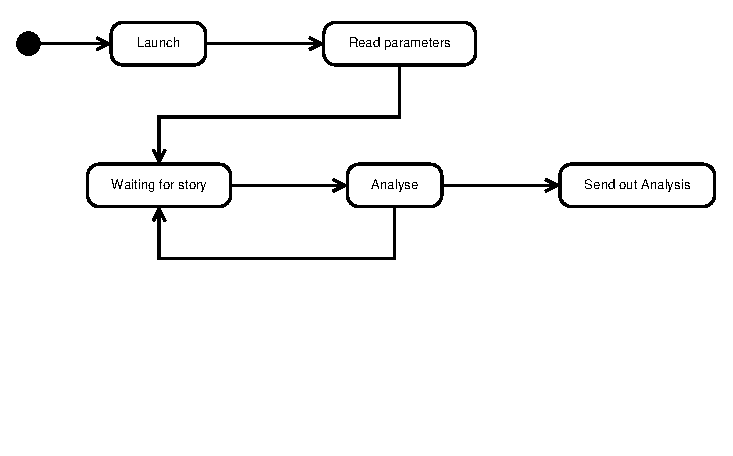
\includegraphics{image/sequence-diagram-sieve}
  \caption{Sequence diagram of a Sieve module}
\end{figure}


\subsection{Life cycle of a ShowOff module}

Upon launch, Launcher parses the command line. It decides that a ShowOff must
be started. This will read the parameters stored in Psyclone. The available
parameter names are:

\begin{itemize}
 \item[Attractors] A comma-separated list of attractors which are specified as
                   $\langle$name$\rangle$:$\langle$weight$\rangle$.
\end{itemize}

After this, the ShowOff goes into a waiting loop, expecting stories and
analyses on their respective whiteboards. When a story is received, a particle
is created, when an analysis is received, the accompanying story is searched
for and the particle is updated accordingly (attraction parameters are
updated).

\begin{figure}[htp]
  \centering
  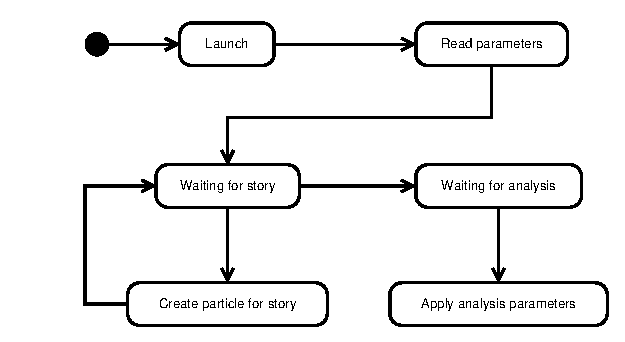
\includegraphics{design/image/sequence-diagram-showoff}
  \caption{Sequence diagram of a ShowOff module}
\end{figure}


\subsection{Life cycle of a Story object}


\subsection{Life cycle of an Analysis object}

An Analysis object is created by Sieve modules. They are created based on an
analysis of a Story object. After the analysis is done, the object is converted
into a \ac{YAML} string and send to the WB.Analyses whiteboard.

Here, it is sent out to all parties interested - ShowOff modules - which
convert the YAML string back into a Analysis object.


\subsection{Life cycle of a Particle object}

\begin{figure}
  \centering
  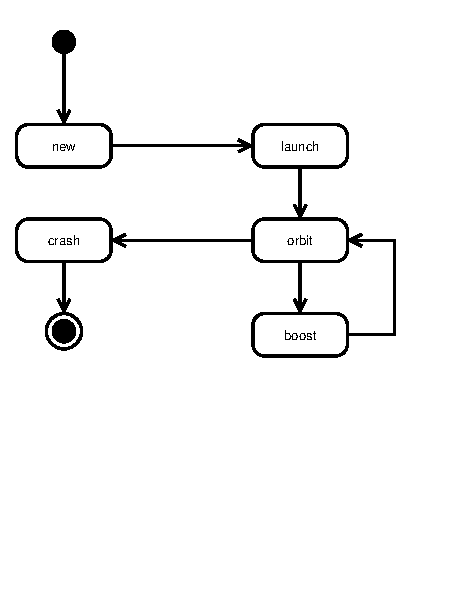
\includegraphics{image/sequence-diagram-particle}
  \caption{The life cycle model of a Particle object}
\end{figure}


